\documentclass[useAMS,usenatbib]{mn2e}
%\documentclass[twocolumn]{emulateapj}
\usepackage{graphicx,natbib,color,multirow,amsmath,url,soul}
\usepackage{epsfig}
\usepackage{float}
\usepackage{deluxetable}
\newcommand{\s}{$_{\rm s}$}
\newcommand{\kms}{km~s$^{-1}$}
\newcommand{\msun}{{\it M}$_{\odot}$}
\newcommand{\lsun}{{\it L}$_{\odot}$}
\newcommand{\mear}{{\it M}$_{\oplus}$}
\newcommand{\etal}{{\it et al.}}
\newcommand{\ie}{{\it i.e.}}
\newcommand{\eg}{{\it e.g.}}
\newcommand{\be}{\begin{equation}}
\newcommand{\ee}{\end{equation}}
\newcommand{\magarc}{{\rm mag\,arcsec$^{-2}$}}
\newcommand{\MK}{{{\rm M}_{\rm ext,K}-5\log h}}
\newcommand{\ri}{{$r_{21}$}}
\newcommand{\ra}{$R_A$}
\newcommand{\vobs}{{v_{\rm obs}}}
\newcommand{\kmsMpc}{km~s$^{-1}$ Mpc$^{-1}$}
\newcommand{\h}{$h_{70}$}
\newcommand{\vpec}{v_{\rm pec}}
\newcommand{\like}{{\mathcal L}}
\newcommand{\vs}{\vspace*{5pt}}
\newcommand{\continued}{ (Continued)}
\newcommand{\radr}{\textsc{petroR90\_r}}


\newcommand{\ferengi}{\textsc{ferengi}}
\newcommand{\hst}{\textit{HST}}
\newcommand{\hubble}{\textit{Hubble Space Telescope}}
\newcommand{\subaru}{\textit{Subaru}}
\newcommand{\sextractor}{\textsc{SExtractor}}
\newcommand{\galapagos}{\textsc{Galapagos}}
\newcommand{\galfit}{\textsc{GALFIT}}
\newcommand{\gimtwod}{\textsc{GIM2D}}
\newcommand{\sersic}{S\'{e}rsic}






% Galaxy Zoo
\newcommand{\ffeatures}{$f_{\rm features}$}
\newcommand{\ffeaturesz}{$f_{\mathrm{features,}z}$}
\newcommand{\ffeaturesrest}{$f_{\mathrm{features,}z=0.3}$}
\newcommand{\ffeaturesdebiased}{$f_{\mathrm{features,debiased}}$}
\newcommand{\fbest}{$f_{\mathrm{features,best}}$}
\newcommand{\fodd}{$f_{\mathrm{odd}}$}
\newcommand{\fbar}{$f_{\mathrm{bar}}$}
\newcommand{\fclumpy}{$f_{\mathrm{clumpy}}$}
\newcommand{\fsmooth}{$f_{\rm smooth}$}
\newcommand{\fartifact}{$f_{\rm artifact}$}

\newcommand{\fHI}{f_{\rm HI}}
\newcommand{\zsim}{$z_{\mathrm{sim}}$}

% Bands

\newcommand{\Bband}{$B_{435W}$}
\newcommand{\Vband}{$V_{606W}$}
\newcommand{\iband}{$i_{775W}$}
\newcommand{\Iband}{$I_{814W}$}
\newcommand{\zband}{$z_{850LP}$}

% GZH subsamples

\newcommand{\main}{\texttt{main}}
\newcommand{\faded}{\texttt{faded}}
\newcommand{\recolored}{\texttt{recoloured}}
\newcommand{\goods}{\texttt{goods-shallow}}
\newcommand{\stripe}{\texttt{stripe-82-single}}
\newcommand{\coadd}{\texttt{stripe-82-coadd}}
\newcommand{\redshifted}{\texttt{redshifted}}
\newcommand{\simagn}{\texttt{simulated-agn}}




\newcommand\ion[2]{[#1$\;${\scshape{#2}}]}      % ion, i.e., [CII] = \ion{C}{ii}
\newcommand\pfeatures{$p_{\rm{features~or~disk}}$}
\newcommand\plusminus[2]{\genfrac{}{}{0pt}{}{#1}{#2}}
\newcommand\pnotedgeon{$p_{\rm{not~edge-on}}$}
\newcommand\pbar{$p_{\rm{bar}}$}
\newcommand\pnobar{$p_{\rm{no~bar}}$}
\newcommand\gztwo{Galaxy~Zoo~2}
\newcommand\mbh{$M_{\rm{BH}}$}
\newcommand\db{$d_{\rm{B-NB}}$}
\newcommand\fb{$f_{\rm{B>NB}}$}
\newcommand\pasa{PASA}
\voffset-1.25cm
\begin{document}

\title[Galaxy~Zoo: passive disk fraction]{Galaxy~Zoo~Hubble: the evolution of red disk galaxies since $z=1$}
\author[Galloway et~al.]{\parbox[t]{16cm}{Melanie A. Galloway$^1$
\vspace{0.1in} }\\
$^{1}$School of Physics and Astronomy, University of Minnesota, 116 Church St. SE, Minneapolis, MN 55455, USA\\
%$^{2}$Wheelock College, Department of Science, Wheelock College, Boston, MA 02215, USA\\
%$^{3}$Institute for Astronomy, Department of Physics, ETH Z\"urich, Wolfgang-Pauli-Strasse 16, CH-8093, Z\"urich, Switzerland\\
%$^{4}$Department of Astronomy and Astrophysics, 1156 High Street, University of California, Santa Cruz, CA 95064, USA\\
%$^{5}$Kavli IPMU (WPI), The University of Tokyo, Kashiwa, Chiba 277-8583, Japan\\
%$^{6}$Oxford Astrophysics, Denys Wilkinson Building, Keble Road, Oxford OX1 3RH, UK\\
%$^{7}$Institute of Cosmology \& Gravitation, University of Portsmouth, Dennis Sciama Building, Portsmouth PO1 3FX, UK\\
%$^{8}$SEPnet --- \url{http://www.sepnet.ac.uk} \\
   }
\maketitle

\begin{abstract}
We study the evolution of the passive disk population from $z=1$ to $z=0.3$ in a sample of 14,000 galaxies from the COSMOS field and morphologically classified by the Galaxy Zoo: Hubble project. We find the fraction of disks occupying the red sequence, as well as the fraction of disk galaxies that are red, to decrease for the most massive galaxies ($\rm log(M/M_{\odot})>11$) but increase for lower masses. Our observations are consistent with a physical scenario in which more massive galaxies are more likely to enter a red disk phase, and more massive red disks are more likely to morphologically transform into ellipticals than their less massive counterparts. This paper also introduces a new method for using artificially-redshifted galaxies to quantify the redshift-bias in Galaxy Zoo classifications in order to accuratly measure the fraction of disk galaxies as a function of redshift.  


\end{abstract}

\section{Introduction}
\label{sec:Intro}

Passive, red disks are an unconventional class of galaxies. They do not adhere to the standard bimodality of the color-morphology relationship, whereby most galaxies tend to exist in one of two populations: blue, late-type disks exhibiting active star formation, and red, early-type ellipticals showing little to no signs of recent star formation \citep{Strateva2001, Baldry2004, Correa2017}. The division between the two populations is particularly apparent when represented visually on a color-magnitude or color color diagram. Galaxies tend to populate in two distinct regions: the ``red sequence'' in the upper band, which contains predominantly early-type galaxies, and the ``blue cloud'' in the lower, containing mostly late-type spirals. This relationship has been shown to hold for $\sim >$ 85\% of galaxies out to z $\sim$ 1 \citep{Bell2004,Cirasuolo2007,Mignoli2009} and possibly beyond \citep{Giallongo2005, vanDokkum2006, Franzetti2007, Cassata2008}. 

The relatively tight correlation between galaxy color (which traces the stellar content) and morphology (which traces dynamical history) suggests an evolutionary link between the two. In the simplest interpretation, it could be deduced that galaxies tend to begin their lives as young, star-forming disks, until some mechanism (secular or external) causes star-formation to cease while the galaxy simultaneously undergoes a morphological transformation from disk to spheroidal. The growing evidence for a significant population of galaxies which breaks this relationship, however, insists on more nuanced interpretations of this model. 

The passive disk population has been a matter of interest for understanding the mechanisms driving the evolutionary link between color and morphology since their initial discovery.  In one of the earliest documented reports of this class, \citet{VandenBergh1976} identified a set of spirals in the Virgo cluster which were forming stars ``much less vigorously'' than the other galaxies of the same type, which were dubbed ``anemic spirals''. Analysis of this population suggested the possibility of ``gentle'' quenching mechanisms which could shut off star-formation without disrupting the morphology (in contrast to violent processes such as mergers, which are capable of destroying the disk \citep{Bell2004,Negroponte1983,DeLucia2006,Springel2005}). The low gas content in the anemic spirals suggested that subtle environmental factors played a role in stripping the gas required to continue star-formation, a process commonly known now as ram-pressure stripping \citep{Gunn1972,Steinhauser2016}. 

Other studies have since investigated other possible mechanisms could lead to the formation of passive disks, and how significant of a contribution this population makes to understanding the full picture of galaxy evolution. Environment is believed to play a strong role in thier formation; many studies for instance find passive spirals preferentially in high-density environments \citep{Dressler1999, Poggianti1999, Goto2003, Deng2009, Hughes2009}. \citet{Moran2006} model the star-formation histories of passive spirals at $z\sim0.4$ and find them to be consistent with models for spirals affected by gas-starvation \citep{Larson1980, Quilis2000, Bekki2002}. Environment plays a significant factor in this scenerio, wherby the interaction of the galaxy with the intra-cluster medium halts the accretion of gas onto the galaxy, inhibiting star-formation and causing a quench without disrupting the morphology significantly. Their results did not argue that starvation was the only mechanism responsible for building up the population of disks in the red sequence, but do conclude that passive disks are indeed an important transition population.

\citet{Masters2010} is one of the few studies which finds no strong correlation of passive disks with environment, but do not rule out environment playing a significant contribution in their creation. They also find strong evidence for quenching via completely secular processes; given by their sample of passive disks being more massive and having a higher bar fraction than their star-forming counterparts. Massive galaxies are more likely to have been assembling for very long times, allowing sufficient time to use up all of their gas, without environment being a direct factor. This option could explain the observed correlations with density and passivity, given that higher-density regions were more likely to have been assembled at earlier times. Secondly, \citet{Masters2010} observed a significantly higher bar fraction in passive spirals (67\%) than star-forming spirals (27\%). Bars are known for their ability to efficiently drive gas to the centers of galaxies via a redistribution of angular momentum throughout the disk \citep{Sellwood1993,Shlosman1989,Ann2005}, which could increase central star-formation \citep{Hawarden1986,Ho1997} or feed the central supermassive black hole \citep{Athanassoula1992,Friedli1993}. The excess of bars in passive disks then suggests that bars were responsible for quickly using up the gas in the galaxy, resulting in subsequent quenching. 

Passive disks have thus far been proposed as both a final stage of galactic evolution, driven by secular and external processes capable of exhausting gas required for star-formation, and as a transition phase of galaxies toward a final evolution to red spheroidal, driven by processes which quench and morphologically transform on different timescales, or multiple separate processes acting independently. Understanding the significance of the passive disk population is therefore unquestionably an important key to understanding galaxy evolution as a whole. \citet{Bundy2010} investigates this subject by measuring the different morphological contributions to the red sequence since $z=1$, and estimate as high as 60\% of all galaxies go through a passive disk phase. It was not quantified which of these further evolve to spheroidal and which stay disks for the remainder of their lifetimes, but the decaying contribution of passive disks to $z=0.3$ was evidence that some fraction of these did indeed transform to elliptical.

This paper will investigate the evolution of the passive disk population from $z=1$ to $z=0.3$ using galaxies identified in the COSMOS field with morphological classifications from Galaxy Zoo: Hubble. We will measure the fraction of disks which are passive and the fraction of the red sequence occupied by disks as functions of mass and redshift, and argue that three factors drive the evolution of these fractions: 1) the rate of blue disks quenching to form passive disks, 2) the rate of blue disks quenching and simultaneously transforming to elliptical, 3) the rate of red disks transforming to red ellipticals, and 4) the net merger rate of ellipticals. We will implement a simple toy model to simulate the evolution of the relative abundances of red disks, blue disks, and red ellipticals, in order to quantify these rate parameters. We will use the results to estimate the fraction of galaxies that enter a red disk phase, and discuss the likelihoods of the red disk phase being a transitory stage or an end-point of a typical galaxy's evolutionary path.

Section~\ref{sec:Data} will describe our methods for selecting disk galaxies and separating the sample into active / passive populations using a color-color diagnostic. In Section~\ref{sec:correction} we describe a new method of correcting for redshift bias in the detection of disk galaxies with Galaxy Zoo classifications using an artificially-redshifted set of images. In Section~\ref{sec:results} we present our results of the fraction of disk galaxies which are red, and the fraction of red sequence galaxies that are disks, as functions of mass and redshift. Here we also explain our toy-model for measuring the dominant evolutionary pathways taken by galaxies in different bins of mass. We compare our findings with results from the literature and discuss their implications in Section~\ref{sec:Discussion}. Our main conclusions are outlined in Section~\ref{sec:conclusions}. We adopt a $\Lambda$CDM cosmology throughout this paper of $\Omega_m=0.31$ and $H_0=68~\rm km~s^{-1} Mpc^{-1}$ \citep{PlanckCollaboration2015}.


\section{Data}
\label{sec:Data}

The parent sample of galaxies in this paper is drawn from the Galaxy Zoo: Hubble (GZH) catalog \citep{Willett2016}, which provides morphological classifications for galaxies sourced from the HST Legacy Surveys. From the main catalog we select galaxies with imaging from the Cosmic Evolution Survey (COSMOS, \citet{Scoville2007}) in the redshift range $0<z<1$.  Rest frame NUV-r and r-J colors are taken from the UltraVISTA catalog \citep{McCracken2012,Ilbert2013}.

\subsection{Sample Selection}
\label{sec:sampleselection}
We identify a sample of 14,663 disk and elliptical galaxies using the morphological classifications provided by GZH. Mergers and irregulars are excluded from the analysis by applying cuts of $\rm f_{irregular} > 0.3$ and $\rm f_{merger} > 0.5$ for galaxies which have at least 20 ``yes'' votes for the question, ``Is there anything odd?''. Last, we apply an inclination limit using $f_{\rm not~edge-on} > 0.3$ and $N_{\rm not~edge-on}>10$. Before applying this cut, it was observed that the red sequence region of the sample was dominated by highly-inclined galaxies, shown in Figure~\ref{fig:edgeon}. Given that galaxy color should be independent of the angle in which it is observed, it is clear that the inclined galaxy colors are strongly affected by dust-reddening. While we are not using dust-corrected colors in our color-color separation, inclination has shown to have an affect on colors even in those which dust-corrected has been attempted \citep{Morselli2016a,Devour2017}. By limiting the sample to face-on galaxies, this bias should be removed (right panel of Figure~\ref{fig:edgeon}). 
 
\begin{figure}
\centering
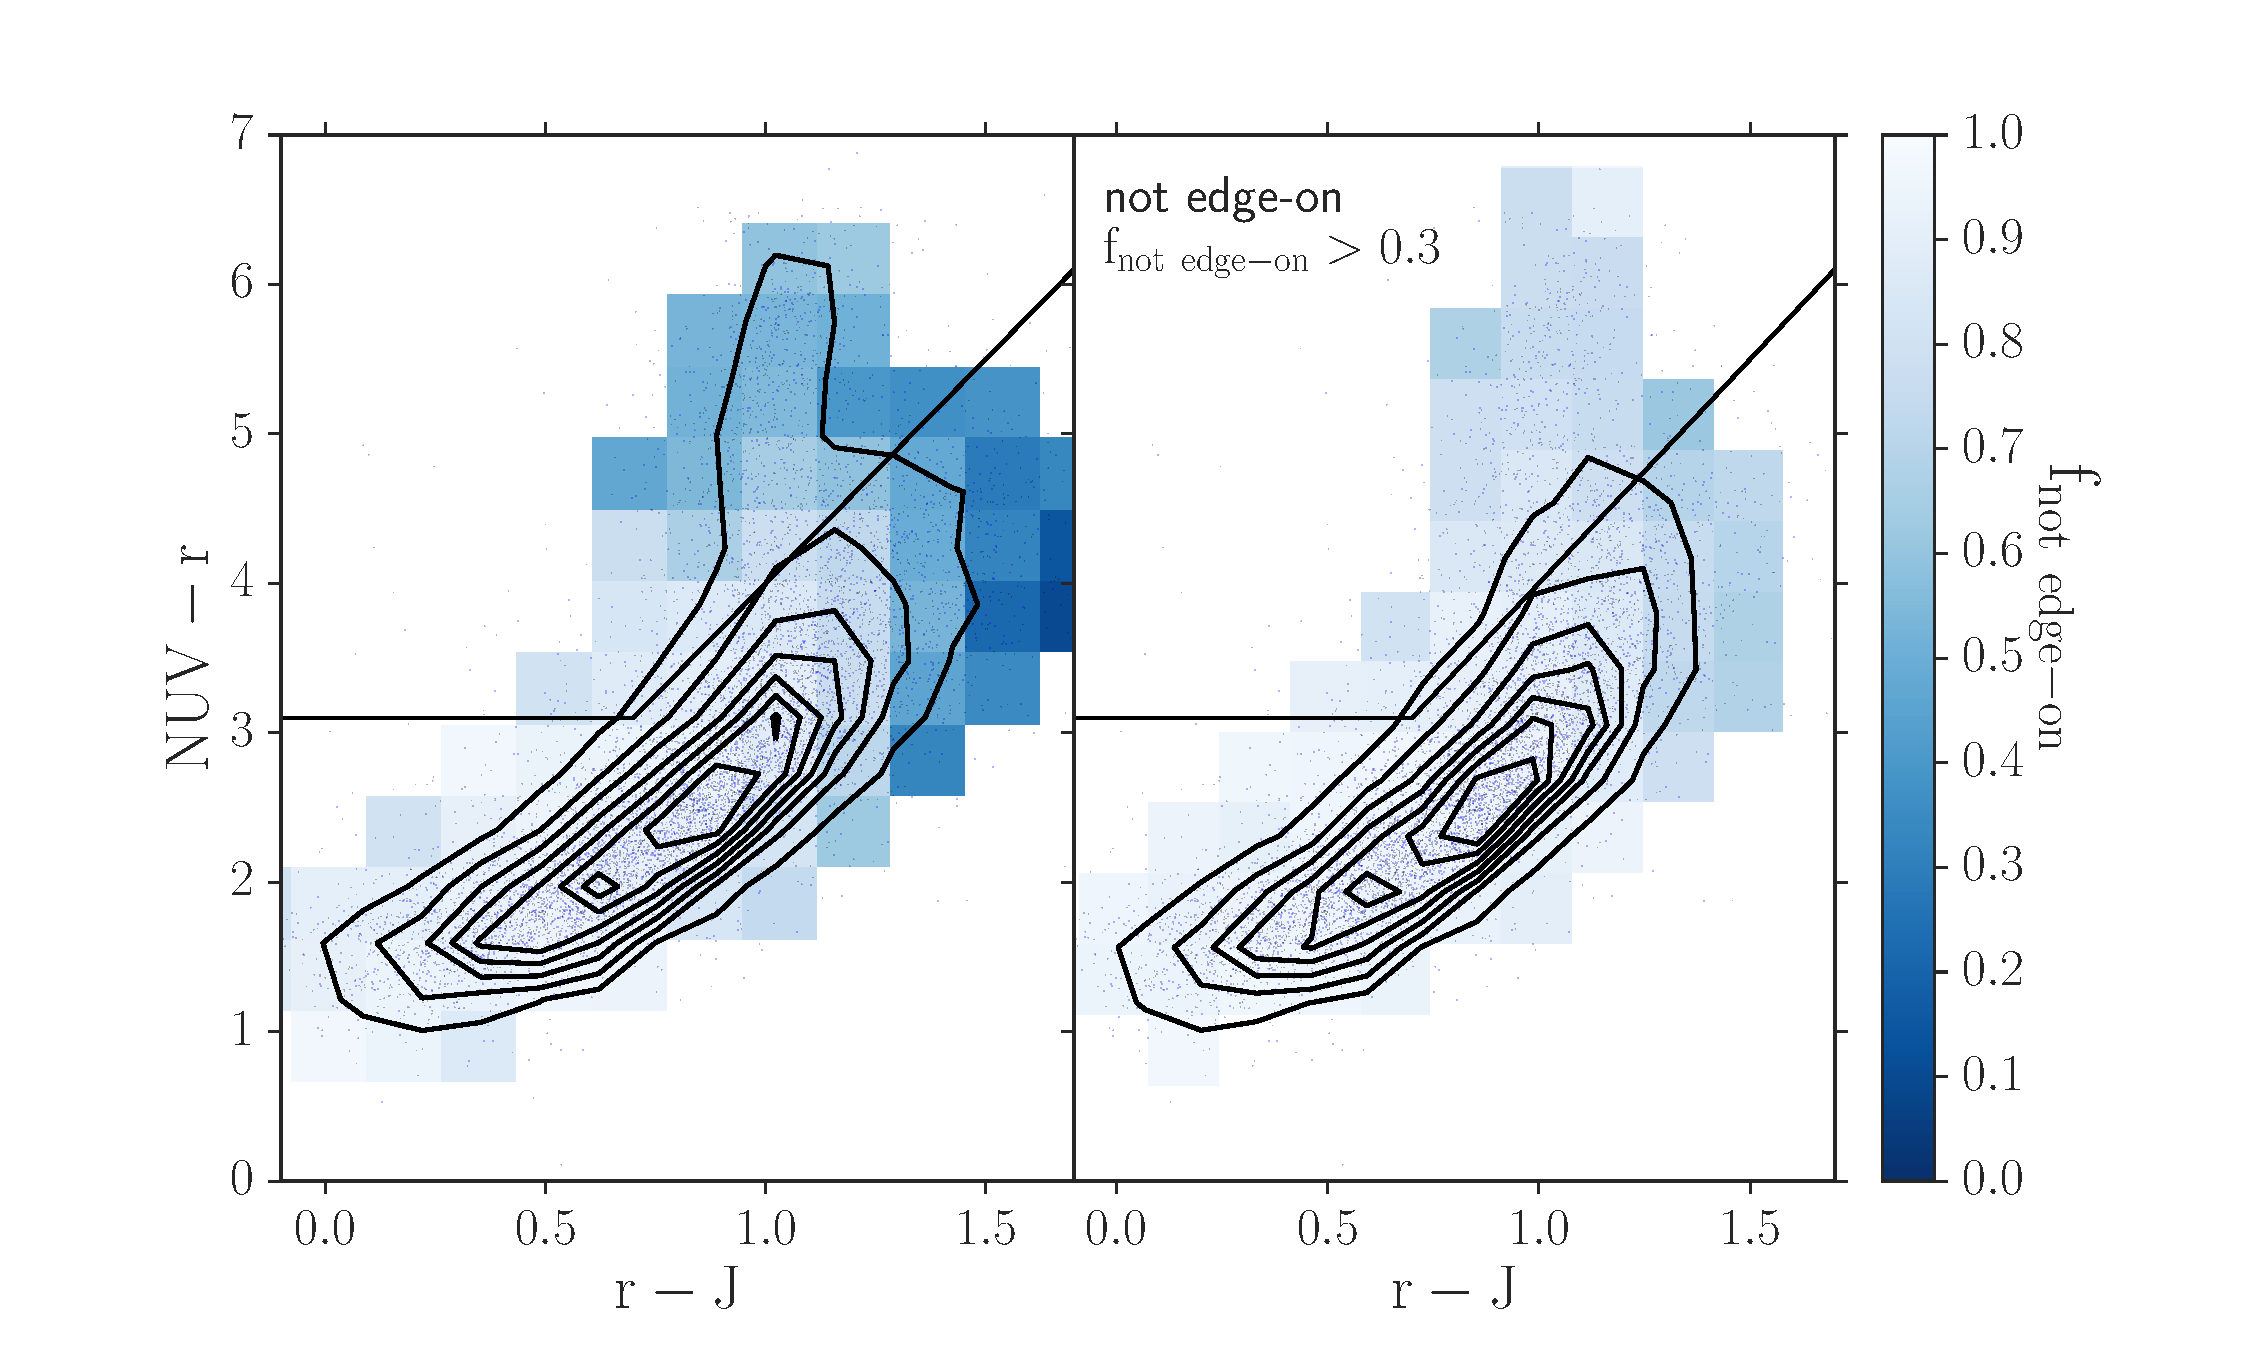
\includegraphics[width=3.5in,trim={1cm 0cm 1cm 1cm},clip]{figures/edgeon_colorcolor.pdf}
\caption{The effect of reddening for highly inclined galaxies. On the left panel is the distribution of $\rm f_{edge-on,no}$, which is the fraction of Galaxy Zoo users who voted ``no'' in response to the question ``Could this be a galaxy viewed edge-on?''. This vote correlates with inclination angle, such that low values represent highly inclined galaxies, and high values represent face-on galaxies. The bins are colored such that darker blue bins have a higher fraction of highly inclined galaxies, and white bins have high fractions of face-on galaxies. There is an obvious bias towards redder colors for galaxies with high inclination angles (low votes for $\rm f_{edge-on,no}$). We therefore implement a cut of $\rm f_{edge-on,no}>0.3$ to ensure that observed red colors are an indicator of a lack of star-formation, and not dust-reddening.[Note: I'm not sure the right panel is particularly useful; it's really just showing the distribution is mostly smoothed out after setting the cut. Keep?] }
\label{fig:edgeon}
\end{figure}
To classify the galaxies as quiescent or star-forming, a method similar to that described by \citet{Ilbert2013} (hereafter I13) was used, which implements a rest-frame NUV-$r$ versus $r$-J diagnostic. Here are some reasons these colors are great (NUV-r:) \citep{Arnouts2007a,Salim2005a,Wyder2007},\citep{Martin2007}

The demarcation line to separate the quiescent and active populations at $z=1$ is adopted from I13, which defines the quiescent galaxies as those which satisfy: $M_{NUV}-M_{r} > 3(M_{r}-M_{J})+1$ and $M_{NUV}-M_{r} > 3.1$. I13 applies this criteria to all galaxies in a range of $0.2<z<3$, although it performs best at separating the two populations in the redshift bin $0.7<z<1.2$, where $>98\%$ of galaxies identified as quiescent exhibited star formation rates less than $log(SFR) = -11$ (see Figure 3 of I13). Therefore this work uses the I13 separation criteria at $z=1$, and computes the evolution of the demarcation lines as a function of redshift to $z=0$. 

The evolution of $r-J$ and $NUV-r$ colors was measured using a stellar population synthesis model from \citet{Bruzual2003}. An instantanious-burst model (ssp) was chosen from the Padova1994 track to represent the color evolution of a passively evolving galaxy, with a metallicity $Z=0.008=.4Z_{\sun}$, which is the typical metallicity of passive galaxies with mass $9 < log(M_{*}/M_{\odot}) < 10$ (\citet{Peng2015}, Figure 2a), chosen to correspond to the median mass of the sample ($log(M_{*}/M_{\odot})=9.7)$. A linear fit was geenerate for each color within the range $0<z<2$, and the slopes for each were used to redefine the demarcation lines in five redshift bins: one with central value $z=0.007$ (used to classify the SDSS ferengi2 sample), and four with central values $z$ = [0.30,0.50,0.70,0.90] with widths $\Delta z=0.2$. The quiescent galaxies are thus defined in these bins as those that satisfy:

\begin{equation}
M_{NUV}-M_{r} > 3.1 + a_{1}(z)
\end{equation}

\begin{equation}
M_{NUV}-M_{r} > 3(M_{r}-M_{J} + a_{2}(z))+ a_{1}(z) + 1  
\end{equation}

where $a_{1}(z) = [0.54,0.38,0.27,0.16,0.05]$ and $a_{2}(z) = [0.19,0.14,0.10,0.06,0.02]$. 
% Figure - mag vs. z (needed??? questionable. useful? also questionable. ) 
%\begin{figure}
%\centering
%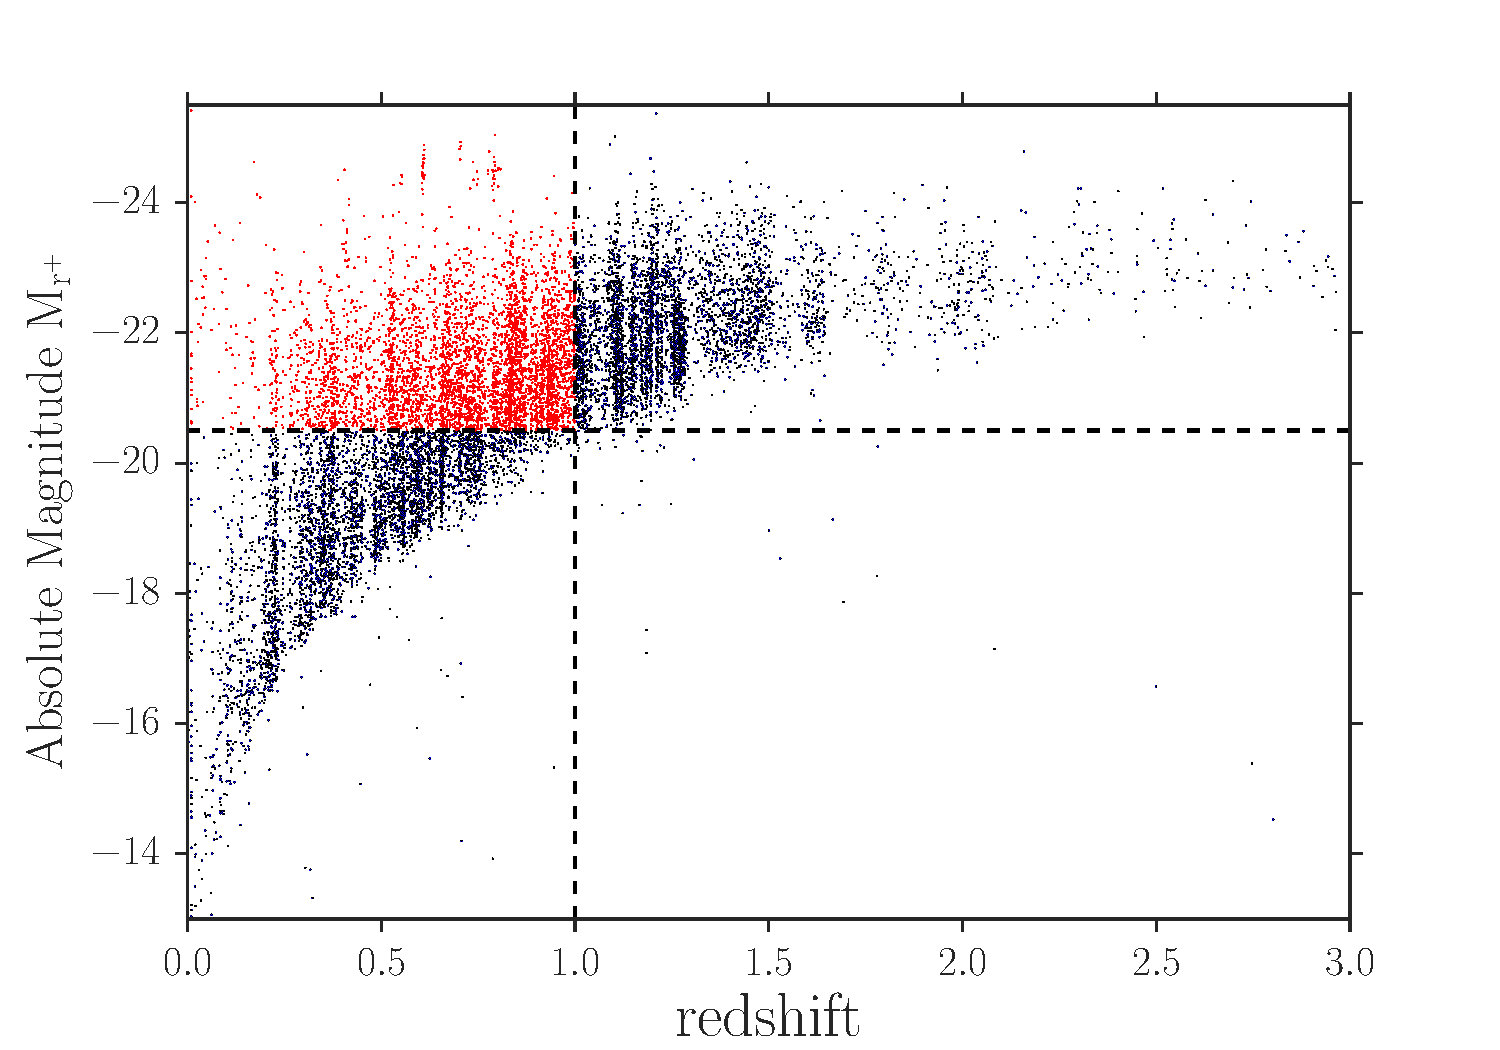
\includegraphics[width=3in]{figures/mag_z_limit.pdf}
%\caption{70,198 COSMOS galaxies cross-matched in GZH and UltraVISTA (all points). 27,584 are in volume-limited sample (red points).}
%\label{fig:volume_lim}
%\end{figure}   

We note that the evolution of the demarcation lines from $z=1$ to $z\sim0$ is very minimal, and our final results do not change if we perform the separation using static lines.


In describing our methods for separating active and passive populations using a color-color separation technique, we have used terminology such that blue/red have been used to describe colors explicitely, while active/passive have been used to describe ongoing/quenched star-formation. The remainder of this paper will assume that the color cuts described in this section adequately separated the active and passive populations, and for convenience the terms red/blue will be used interchangeably with passive/active.  

\section{Correcting for Incompleteness in Disk Detection}
\label{sec:correction}
In this work, we study the growth of the red sequence population by evaluating the fraction of passive disks as a function of redshift, $\rm N_{red~disks}/(N_{red~disks}+N_{blue~disks})$, as well as the fraction of disks occupying the red sequence, $\rm N_{red~disks}/(N_{red~disks}+N_{red~ellipticals})$. To accurately measure these fractions, the number of disks and ellipticals populating each redshift interval must be known with confidence. To identify disk galaxies in our sample, we set a cut of $f_{\rm features}\ge0.3$, such that galaxies meeting this criteria are considered to have distinguishable features or disk structure (additional cuts are also placed to eliminate clumpy, highly inclined, and merging galaxies; see Section~\ref{sec:sampleselection}), and galaxies which do not are considered elliptical. However, it is known that distinguishing disk structure from spheroidal becomes increasingly challenging at high redshifts (for both experts and novice classifiers alike), where features are less resolved and more difficult to identify. \citet{Willett2016} show using a set of artificially-redshifted simulated galaxy images classified in Galaxy Zoo that vote fractions for the same galaxy can be drastically different measured at $z=1$ from $z=0$, often enough to change its morphological classification (we will show the same in Section~\ref{ssec:ferengi}).  Therefore it is predicted that applying a $f_{\rm features}$ cut to identify disks will increasingly underestimate their true number at increasing redshift intervals. A set of artificially redshifted images was used to quantify and correct for this incompleteness in disk and elliptical detection, described in the next section.
 
\subsection{FERENGI2 set of artificially redshifted galaxy images}
\label{ssec:ferengi}
\ferengi2 is a set of simulated galaxy images created using the \ferengi{} code \citep{Barden2008}. These were created from a parent sample of 936 nearby ($z<0.01$) SDSS galaxies, all of which had been previously classified in Galaxy Zoo 2 and were cross-matched in 2MASS \citep{Skrutskie2006} for J magnitudes and GALEX \citep{Martin2005} for NUV magnitudes, which were necessary to create a color-color separation using a method as similar as possible to that of the COSMOS sample.  An evolution factor of $e=-1$ was applied, which brightens each galaxy linearly with redshift: $M' = M + ez$, where $M'$ is the corrected magnitude. This correction is performed to mimic the known physical increase of galaxy magnitude with redshift \citep{Lilly1998,Loveday2011}, and the value $e=-1$ was chosen based on an analysis of spectra template models provided by \citet{Brinchmann2004a}, which showed that typical galaxies tend to evolve in brightness by one magnitude per redshift. Each galaxy was artificially redshifted 8 times from $z=0.3$ to $z=1$ in intervals of $\Delta z = 0.1$ and processed to mimic $HST$ imaging parameters, giving a total of 7,488 images (3 examples are shown in Figure~\ref{fig:ferengi2example}).  The set was then classified in Galaxy Zoo using the same decision tree as used for Galaxy Zoo Hubble. 134 highly inclined disk galaxies were removed from the sample by excluding any with $N_{edgeon}>20$ and $f_{not~edge-on}>=0.6$, using the vote fraction associated with the real galaxy image measured in GZ2. This cut was shown in \citet{Galloway2015} to correlate well with inclination angle $cos(a/b)<67^\circ$. This was to exclude those which may be mis-classified due to dust-reddening.  Using the NUV-J-R selection method described in section~\ref{sec:sampleselection}, the remaining sample was divided into a set of red sequence galaxies (259 per redshift bin) and blue cloud (543 per each redshift bin) (see Figure~\ref{fig:ferengi2colorcolor}).

\begin{figure}
\centering
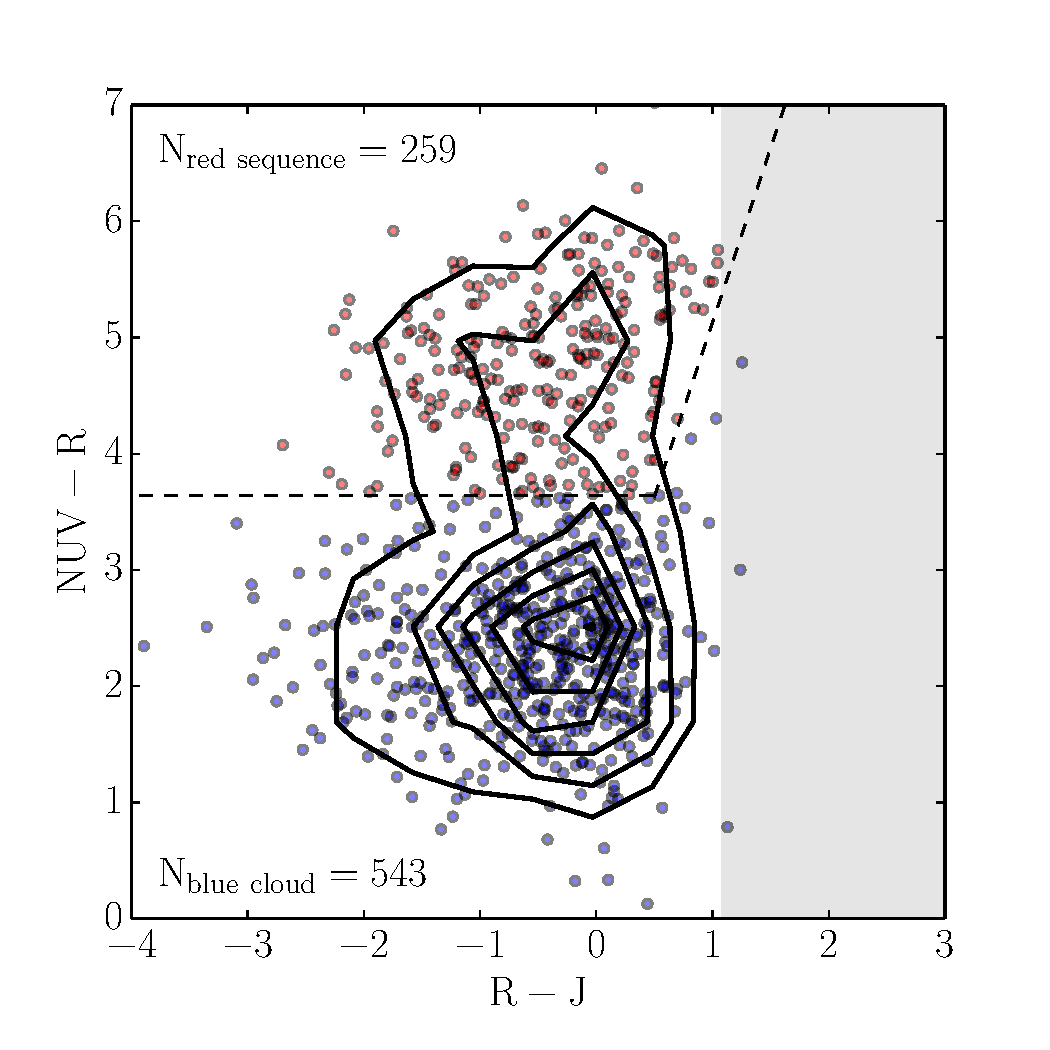
\includegraphics[width=2.5in,height=2.5in,trim={.5cm 0cm .5cm 0cm},clip]{figures/ferengi2_colorcolor.pdf}
\caption{Separation of the quiescent population (red sequence) and active population (blue cloud) of the \ferengi2 sample. The gray shaded region represents the R-J limit of the sample; since \ferengi2 is a subset of GZ2, for which a limit of $r<17$ was implemented, and the magnitude limit of 2MASS is $J<15.91$, the \ferengi2 sample is limited to R-J $<$ 1.1.}
\label{fig:ferengi2colorcolor}
\end{figure}

\begin{figure*}
\centering
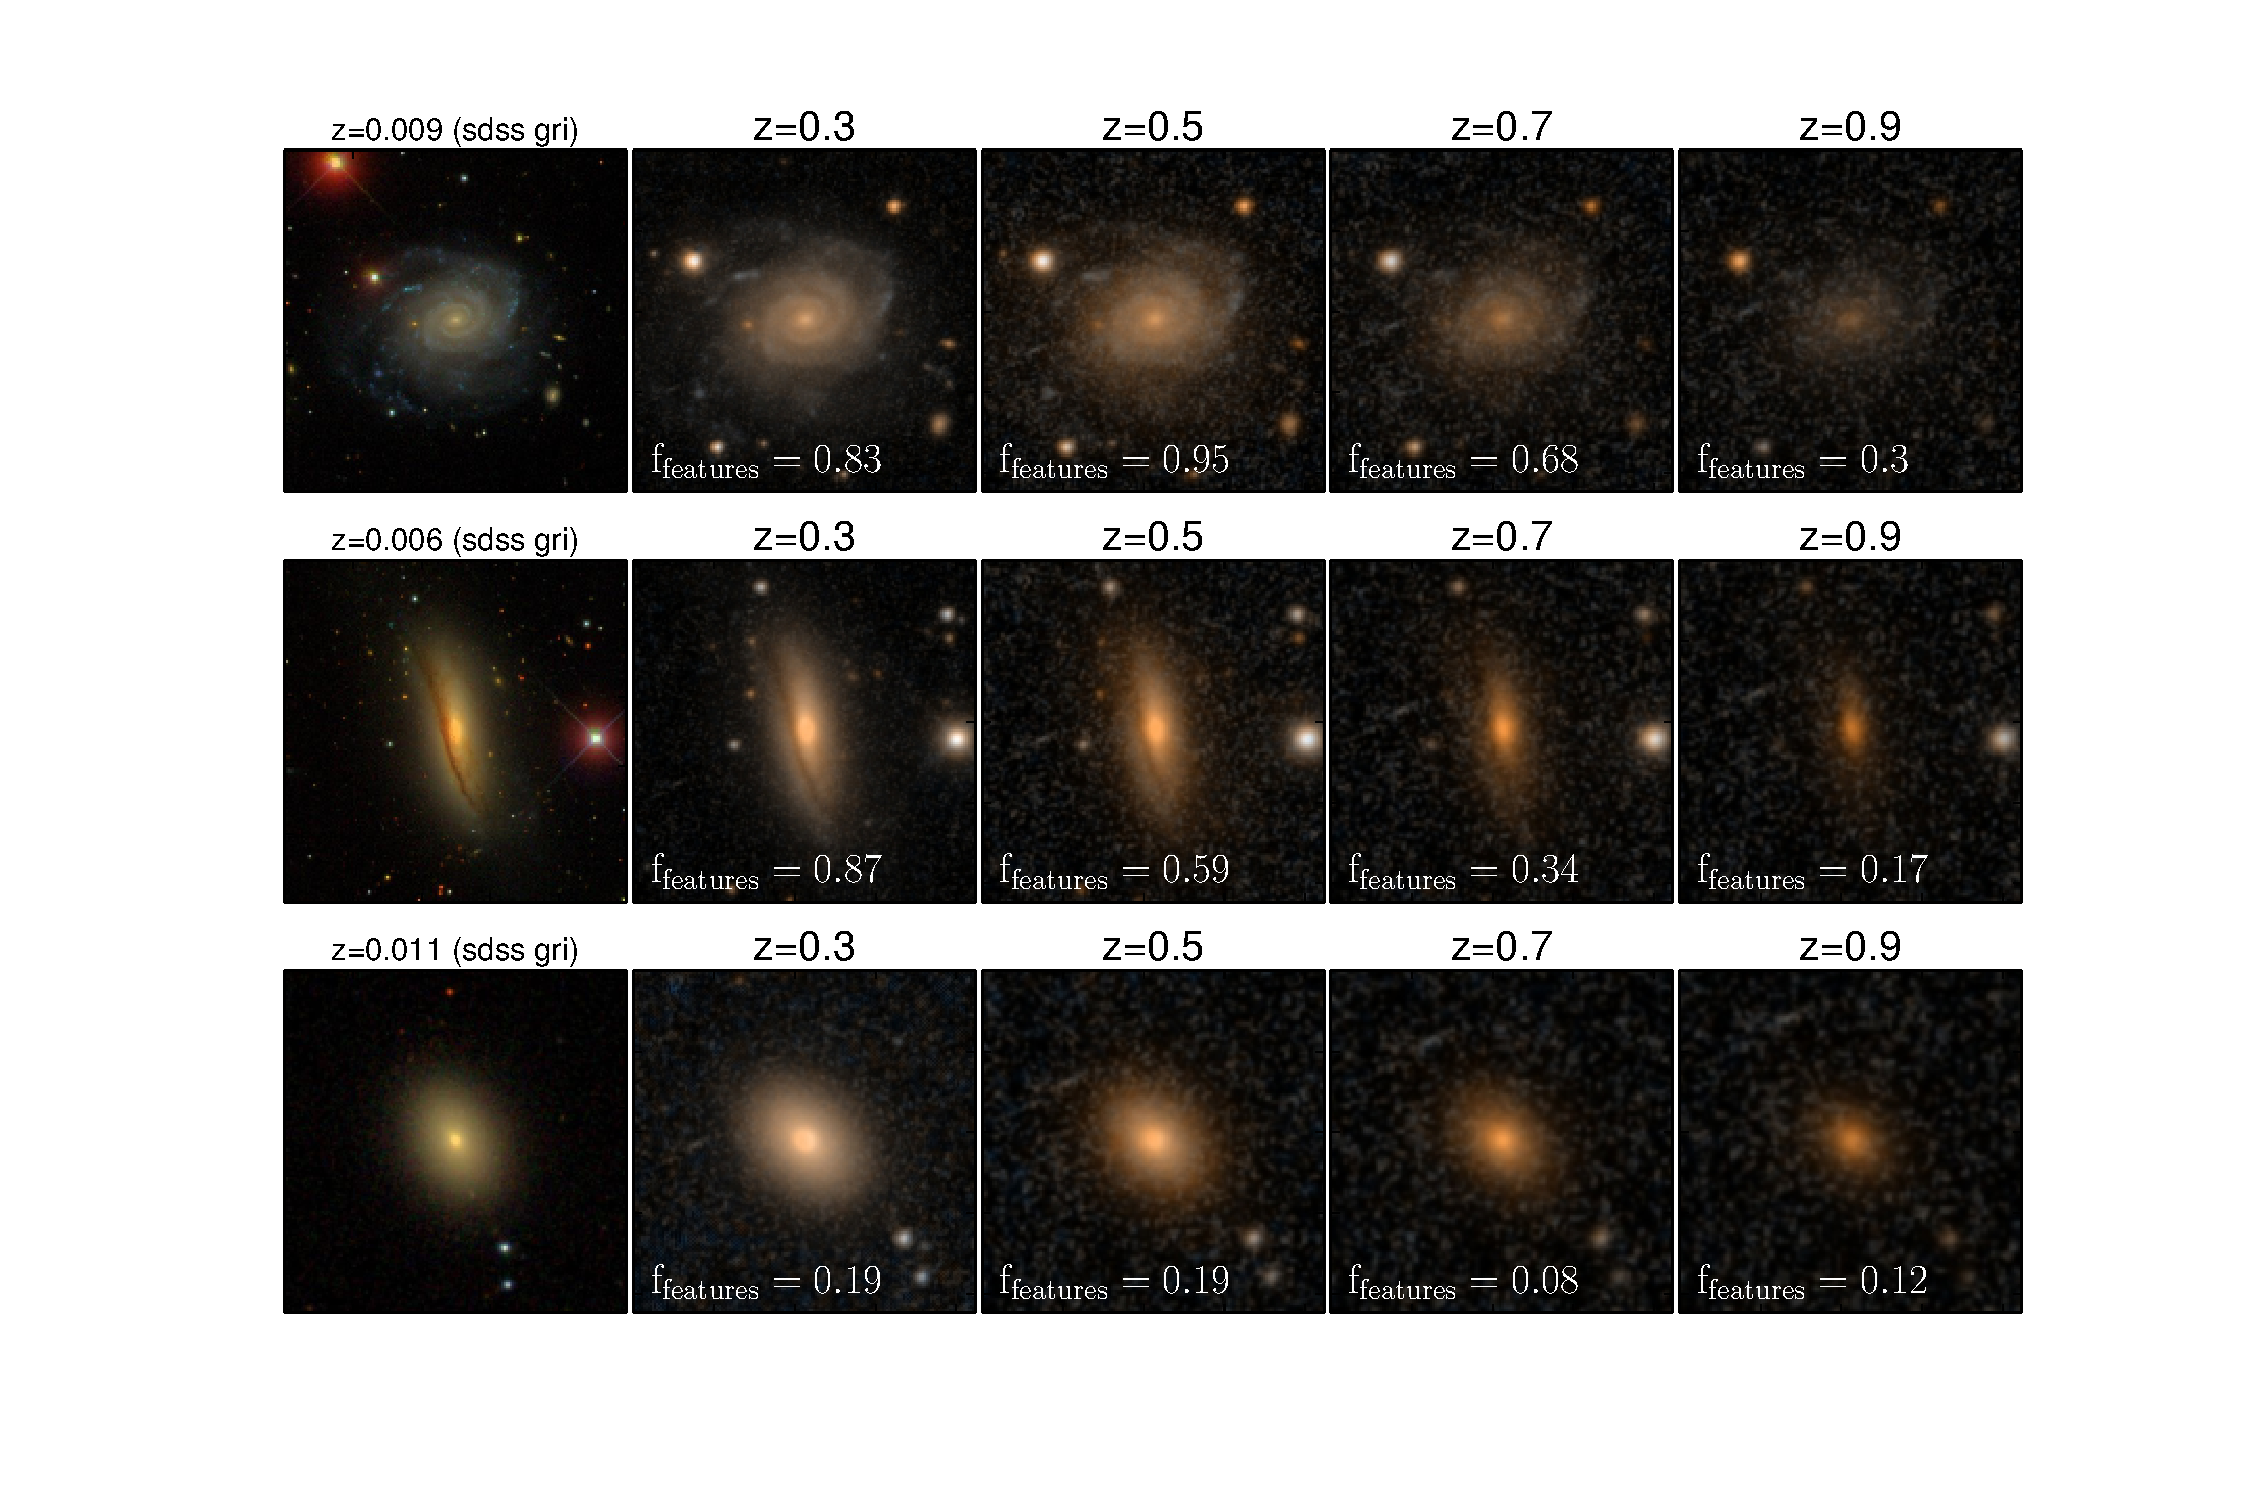
\includegraphics[width=\textwidth,trim={.5cm 3cm .5cm .5cm},clip]{figures/ferengi2_examples_with_fractions.pdf}
\caption{Example images of three galaxies artificially redshifted with the \ferengi{} code. The left image in each row is a real SDSS gri-composite image; the four to the right are images generated by \ferengi{} at varying redshifts, processed to mimic $HST/COSMOS$ imaging. The \ffeatures{} vote fraction for each simulated image is given; this value tends to decrease for each galaxy as it is processed to be viewed at higher redshifts. }
\label{fig:ferengi2example}
\end{figure*}

\subsection{Measuring $\xi$}
\label{ssec:xi}

The \ferengi2 set was used to measure the incompleteness in disk and elliptical detection, from which correction factors $\xi_{disk}$ and $\xi_{ellitpical}$ were derived. These are defined as the number of disks/ellipticals detected divided by the true number of disks/ellipticals expected to exist in a given redshift interval: $\rm \xi_{disk}(z)=N_{disks~detected}/N_{\rm disks~true}$, and $\rm \xi_{elliptical}(z)=N_{ellipticals~detected}/N_{ellipticals~true}$


 Acknowledging that the completeness in disk detection may depend on galaxy color, the corrected fraction of passive disks can then be calculated as:

\begin{equation}
f_{R|D}=\frac{N_{RD}\times \xi^{-1}_{red~disks}}{N_{RD}\times \xi^{-1}_{red~disks} + N_{BD} \times \xi^{-1}_{blue~disks}}
\label{eqn:fdir}
\end{equation}

If there is no color bias in disk detection, $\xi_{red disks}=\xi_{blue disks}$, and this term cancels out, leaving the fraction unchanged. If there is a bias, however, the $\xi$ terms do not cancel, and the incompleteness in disk detection could have a large effect on the red disk fraction. Therefore a careful measurment of $\xi$ is estimated for both red and blue disk galaxies using the \ferengi2 set of simulated images.

The completness values $\xi_{red disks}(z)$ and $\xi_{blue disks}(z)$ were computed in varying bins of redshift for the red sequence and blue cloud galaxies separately. An example calculation of $\xi_{blue disks}$ in the $z=0.7$ bin is shown in Figure~\ref{fig:inc_subplot}. Each point represents a \ferengi2 galaxy, where the y-axis indicates the value of \ffeatures~measured in the image redshifted to $z=0.7$, and the x-axis indicates the value of \ffeatures~measured in the same galaxy redshifted to $z=0.3$. Disk galaxies are identified as those for which \ffeatures~$\ge0.3$. Since, on average, \ffeatures~decreases for the same galaxy as it is viewed at higher redshifts, the number of galaxies meeting this threshold is generally fewer at higher redshifts than lower redshifts. This is indicated by the dotted lines: galaxies to the right of the vertical dashed line at $\rm f_{features,z=0.3}=0.3$ are identified as disks at $z=0.3$; their sum is considered the ``true'' number of disks, $\rm N_{true}$. Similarly, the galaxies above the horizontal line at $\rm f_{features,z=0.7}=0.3$ are identified as disks at $z=0.7$; their sum is the ``detected'' number of disks at $z=0.7$, or $\rm N_{disks detected}$. As obvious in the figure, $\rm N_{disks detected}$ is in general much lower than $\rm N_{disks true}$, emphasizing the increasing difficulty in detecting features at higher redshifts. Their ratio is the completeness $\xi$; in this example $\xi_{blue disks}(z=0.7)=0.61$, meaning only 61\% of disks were detected at this redshift. 

\begin{figure}
\centering
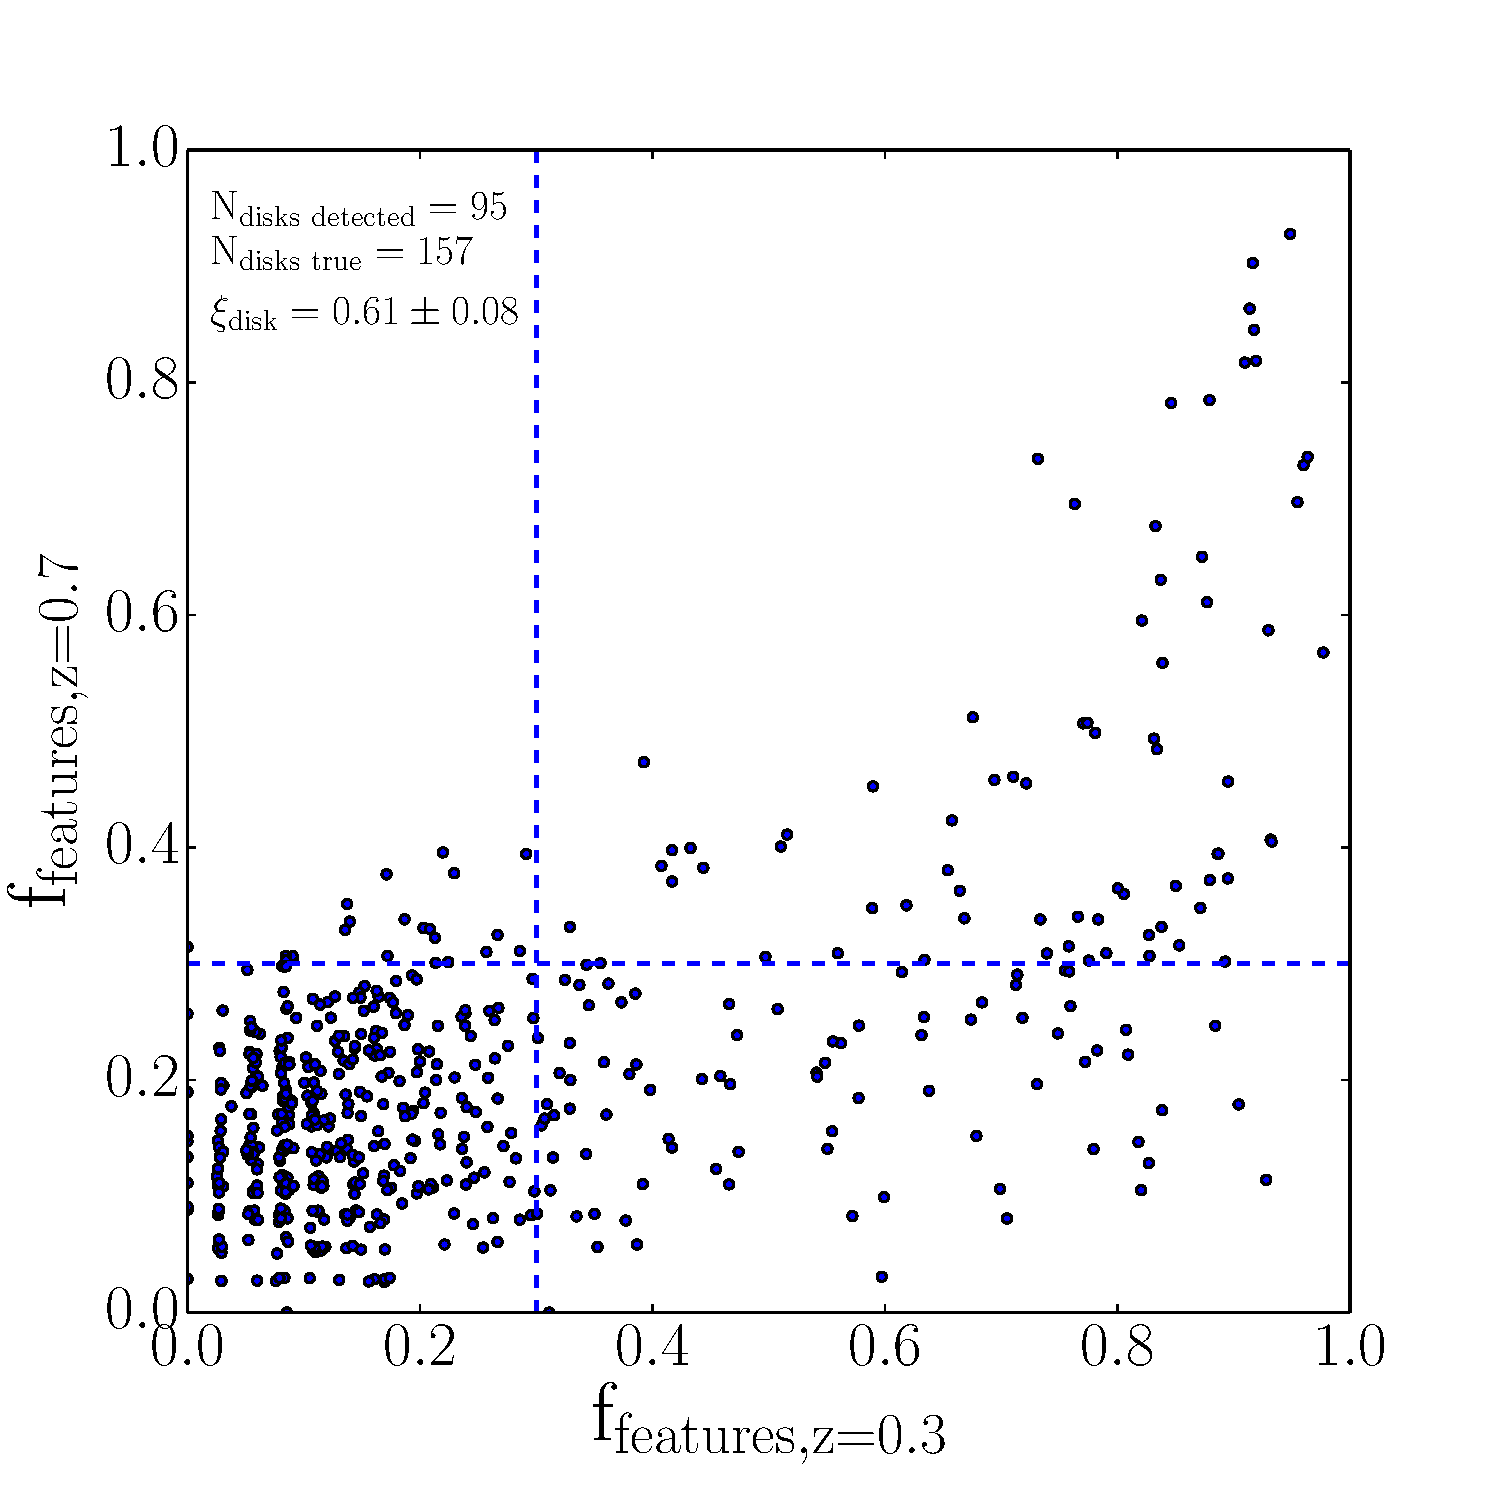
\includegraphics[width=.5\textwidth]{figures/incompleteness_z7.pdf}
\caption{Example calculation of completeness $\xi$ at redshift $z=0.7$. Points represent \ferengi2 images classified in Galaxy Zoo. The y-axis corresponds to the value of \ffeatures~measured at the galaxy redshifted to $z=0.7$, and the x-axis corresponds to the value of \ffeatures~measured at the galaxy redshifted to $z=0.3$. On average, the \ffeatures~is lower at the higher redshift, indicating users on average have more difficulty identifying features in images at higher redshifts. The dotted lines correspond to \ffeatures=0.3, the threshold above which a galaxy is considered to have a disk. Galaxies to the right of the vertical dashed line were identified as disks at the lowest redshift $z=0.3$, the total number defined as $\rm N_{true}$, the true number of disks. Galaxies above the horizontal dash line were identified as disks at the higher redshift $z=0.7$, the total number defined as $\rm N_{disks detected}$. The ratio $\rm \xi=N_{disks detected}/N_{disks true}$ is the completeness value; in this example, only 61\% of disks were detected at $z=0.7$.}
\label{fig:inc_subplot}
\end{figure}

It was hypothesized that the completeness in disk detection may be a function of other parameters in addition to redshift. At fixed redshift, for example, it is reasonable to guess that features could be easier to detect galaxies that have higher mass, radius, or surface brightness. To test whether these parameters also impact the number of disks detected, the completeness was measured in fixed redshift bins as a function of surface brightness, effective radius, and mass. The surface brightness was calculated as $\mu = m + 2.5*\log_{10}{(2 \times (b/a) \times \pi R_e^2 )}$, using \sextractor{} outputs {\tt MAG\_AUTO}, $b/a$ and $R_{e}$ measured in the \Iband{} band images. The effective radius used was the 50\% {\tt FLUX\_RADIUS} converted in to kpc, and the masses used were the {\tt MEDIAN} values in the MPA-JHU DR7 catalog \citep{Kauffmann2003b}.

Figure~\ref{fig:xi_v_sb} shows completeness as a function of redshift and surface brightness, for the red sequence and blue cloud galaxies. 8 redshift bins were further divided into bins of surface brightness with varying widths, where the sizes were chosen to satisfy that $\rm N_{detected} + N_{true} \ge 10$ in each bin. This was chosen as a comprimise between having a sufficient number of galaxies in each bin to compute the completness fraction $\rm \xi = N_{detected}/N_{true}$, and to have enough bins of surface brightness to measure a trend with confidence of completeness as a function of $\mu$. Visual inspection of the data did not suggest any relationship between the two. To be sure, the data were fit to a linear function in each redshift bin. For each fit, a p-value representing a hypothesis test whose null hypothesis is that the slope is zero was computed. Only one reached the criteria $p<0.05$, but with a low $R^{2}$ value of 0.28 which is not considered large enough to represent a good fit. This process was repeated using effective radius and mass as parameters, with the same results. Therefore only redshift was used as a parameter which impacted completeness value with confidence. 

\begin{figure}
\centering
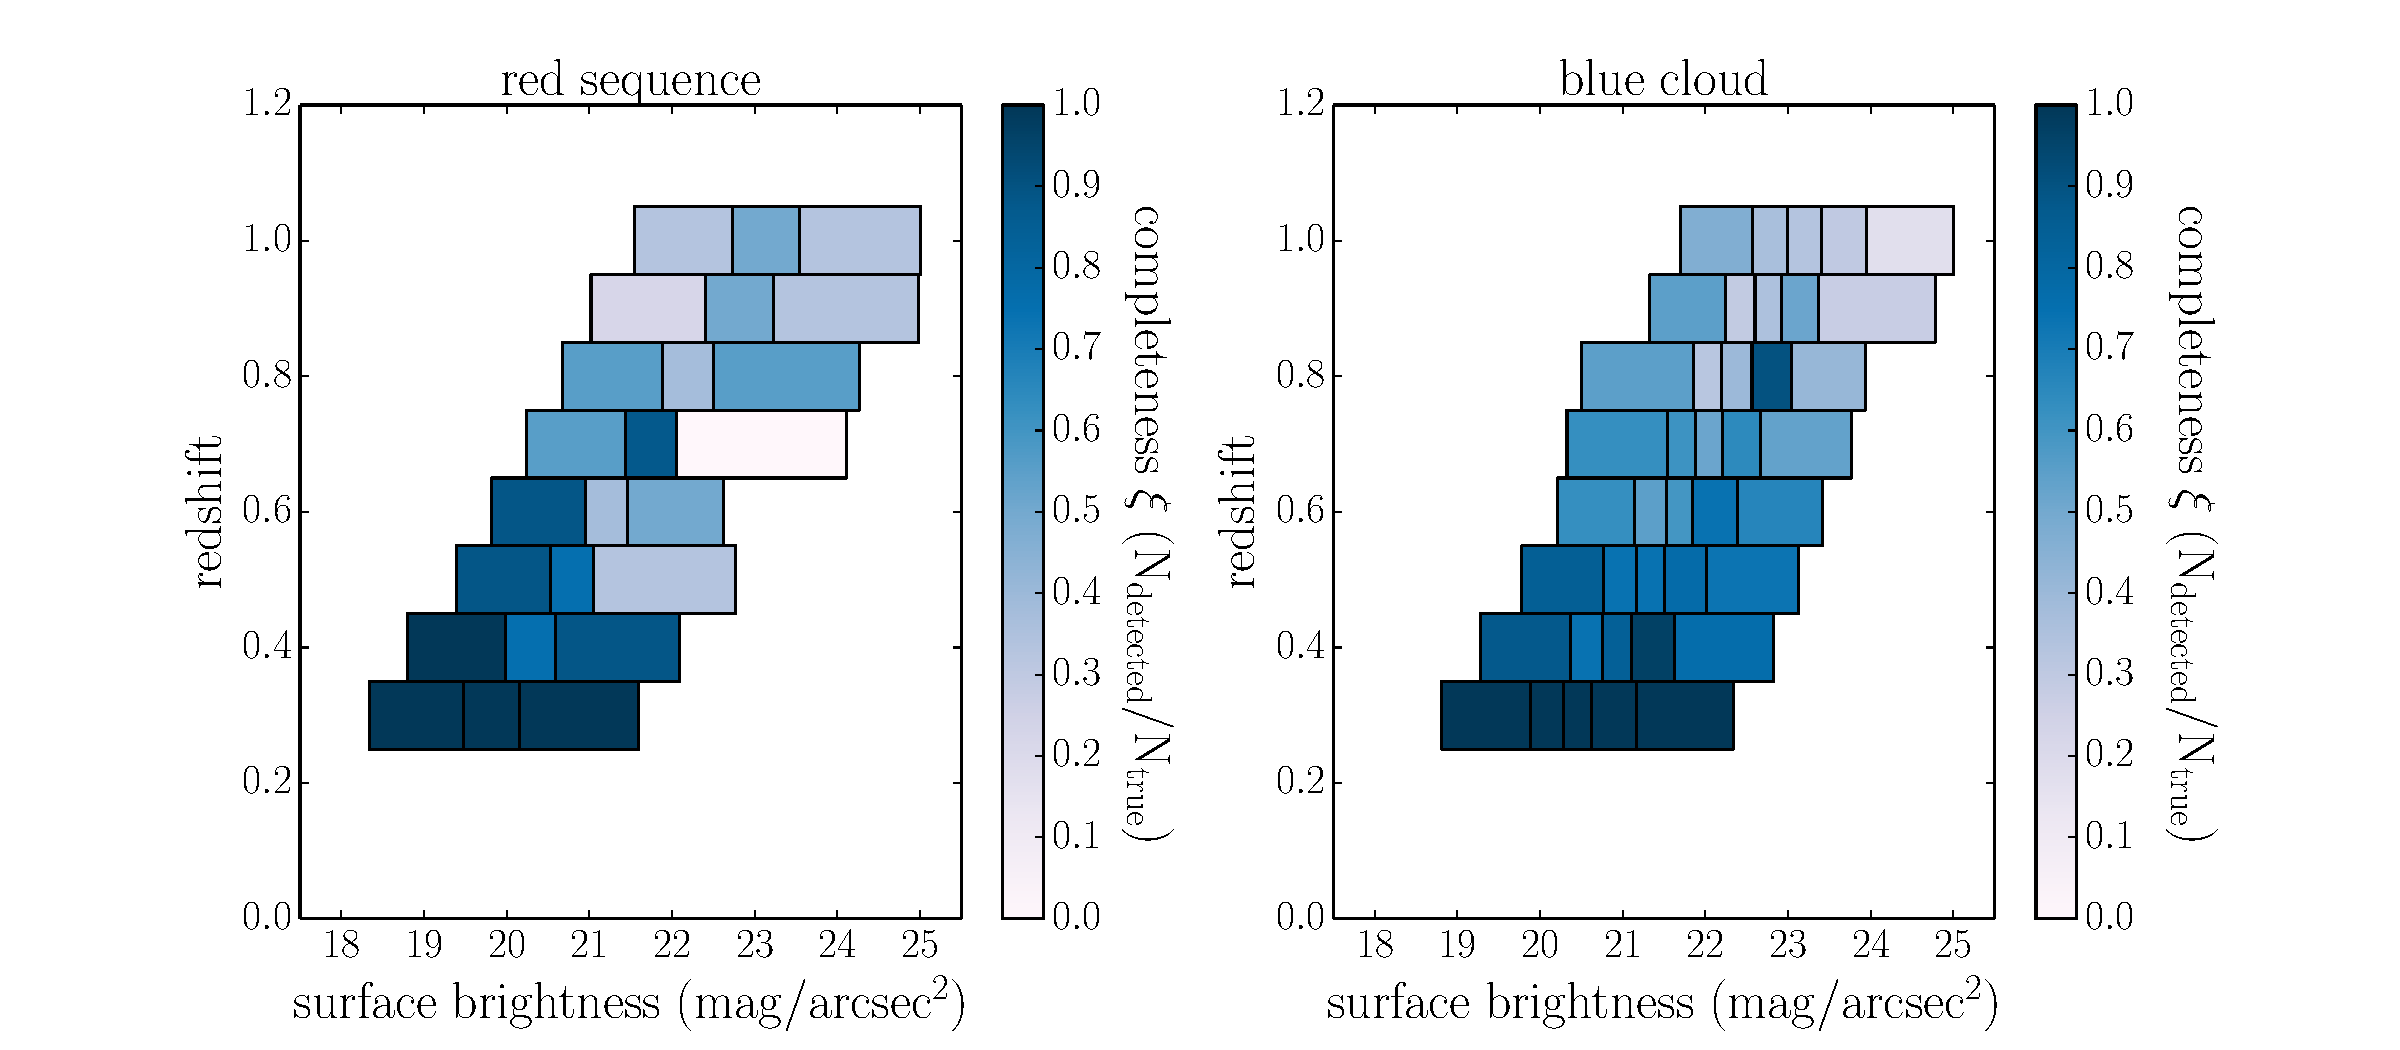
\includegraphics[width=3.5in,trim={3cm 0cm 3cm 0cm},clip]{figures/xi_v_sb.pdf}
\caption{Completeness $\xi$ as a function of redshift and surface brightness for red sequence (left) and blue cloud galaxies (right). In each redshift bin, galaxies were binned by surface brightness in varying widths such that $\rm N_{detected} + N_{true} \ge 10$ in each bin. The completness $\xi$ was computed in each $z,\mu$ bin, represented by the colors. Darker colors represent a completeness of 1, such that all disks were detected, while fainter colors represent a completeness near 0, representing a failure to detect disks. $\xi$ tends to decrease with redshift, but no correlation of $\xi$ with surface brighness is observed at fixed redshift.}
\label{fig:xi_v_sb}
\end{figure}


The completeness values $\rm \xi_{red disks}$ and $\rm \xi_{blue disks}$ were then measured as a function of redshift for the red sequence and blue cloud \ferengi2 galaxies; results are shown in Figure~\ref{fig:xi}. No significant difference was detected for the two functions, which is apparent from the overlapping $1-\sigma$ errors on the plot. The process was then repeated for the elliptical galaxies; as with the disk sample, no dependence on completeness $\xi_{ellipticals}$ with variables other than redshift was found. Therefore $\xi_{disks}$ and $\xi_{ellipticals}$ were computed for all galaxies in bins of redshift between 0.3 and 1.0 with widths $\Delta z = 0.1$; from here linear relationships for $\xi_{disks}$ and $\xi_{ellipticals}$ as functions of redshift were derived: $\xi(z) = -0.9 \pm x (z) + 1.2 \pm y$. These corrections were used to calculate the fractional contribution of each morphological/activity type (Figure~\ref{fig:all_plot}), and the fraction of disks on the red sequence (Figure~\ref{fig:f_results}):

\begin{equation}
f_{D|R}=\frac{N_{RD}\times \xi_{disks}^{-1}}{N_{RD}\times \xi_{disks}^{-1} + N_{RE}\times \xi_{ellipticals}^{-1}}
\label{eqn:frid}
\end{equation}


\begin{figure}
\centering
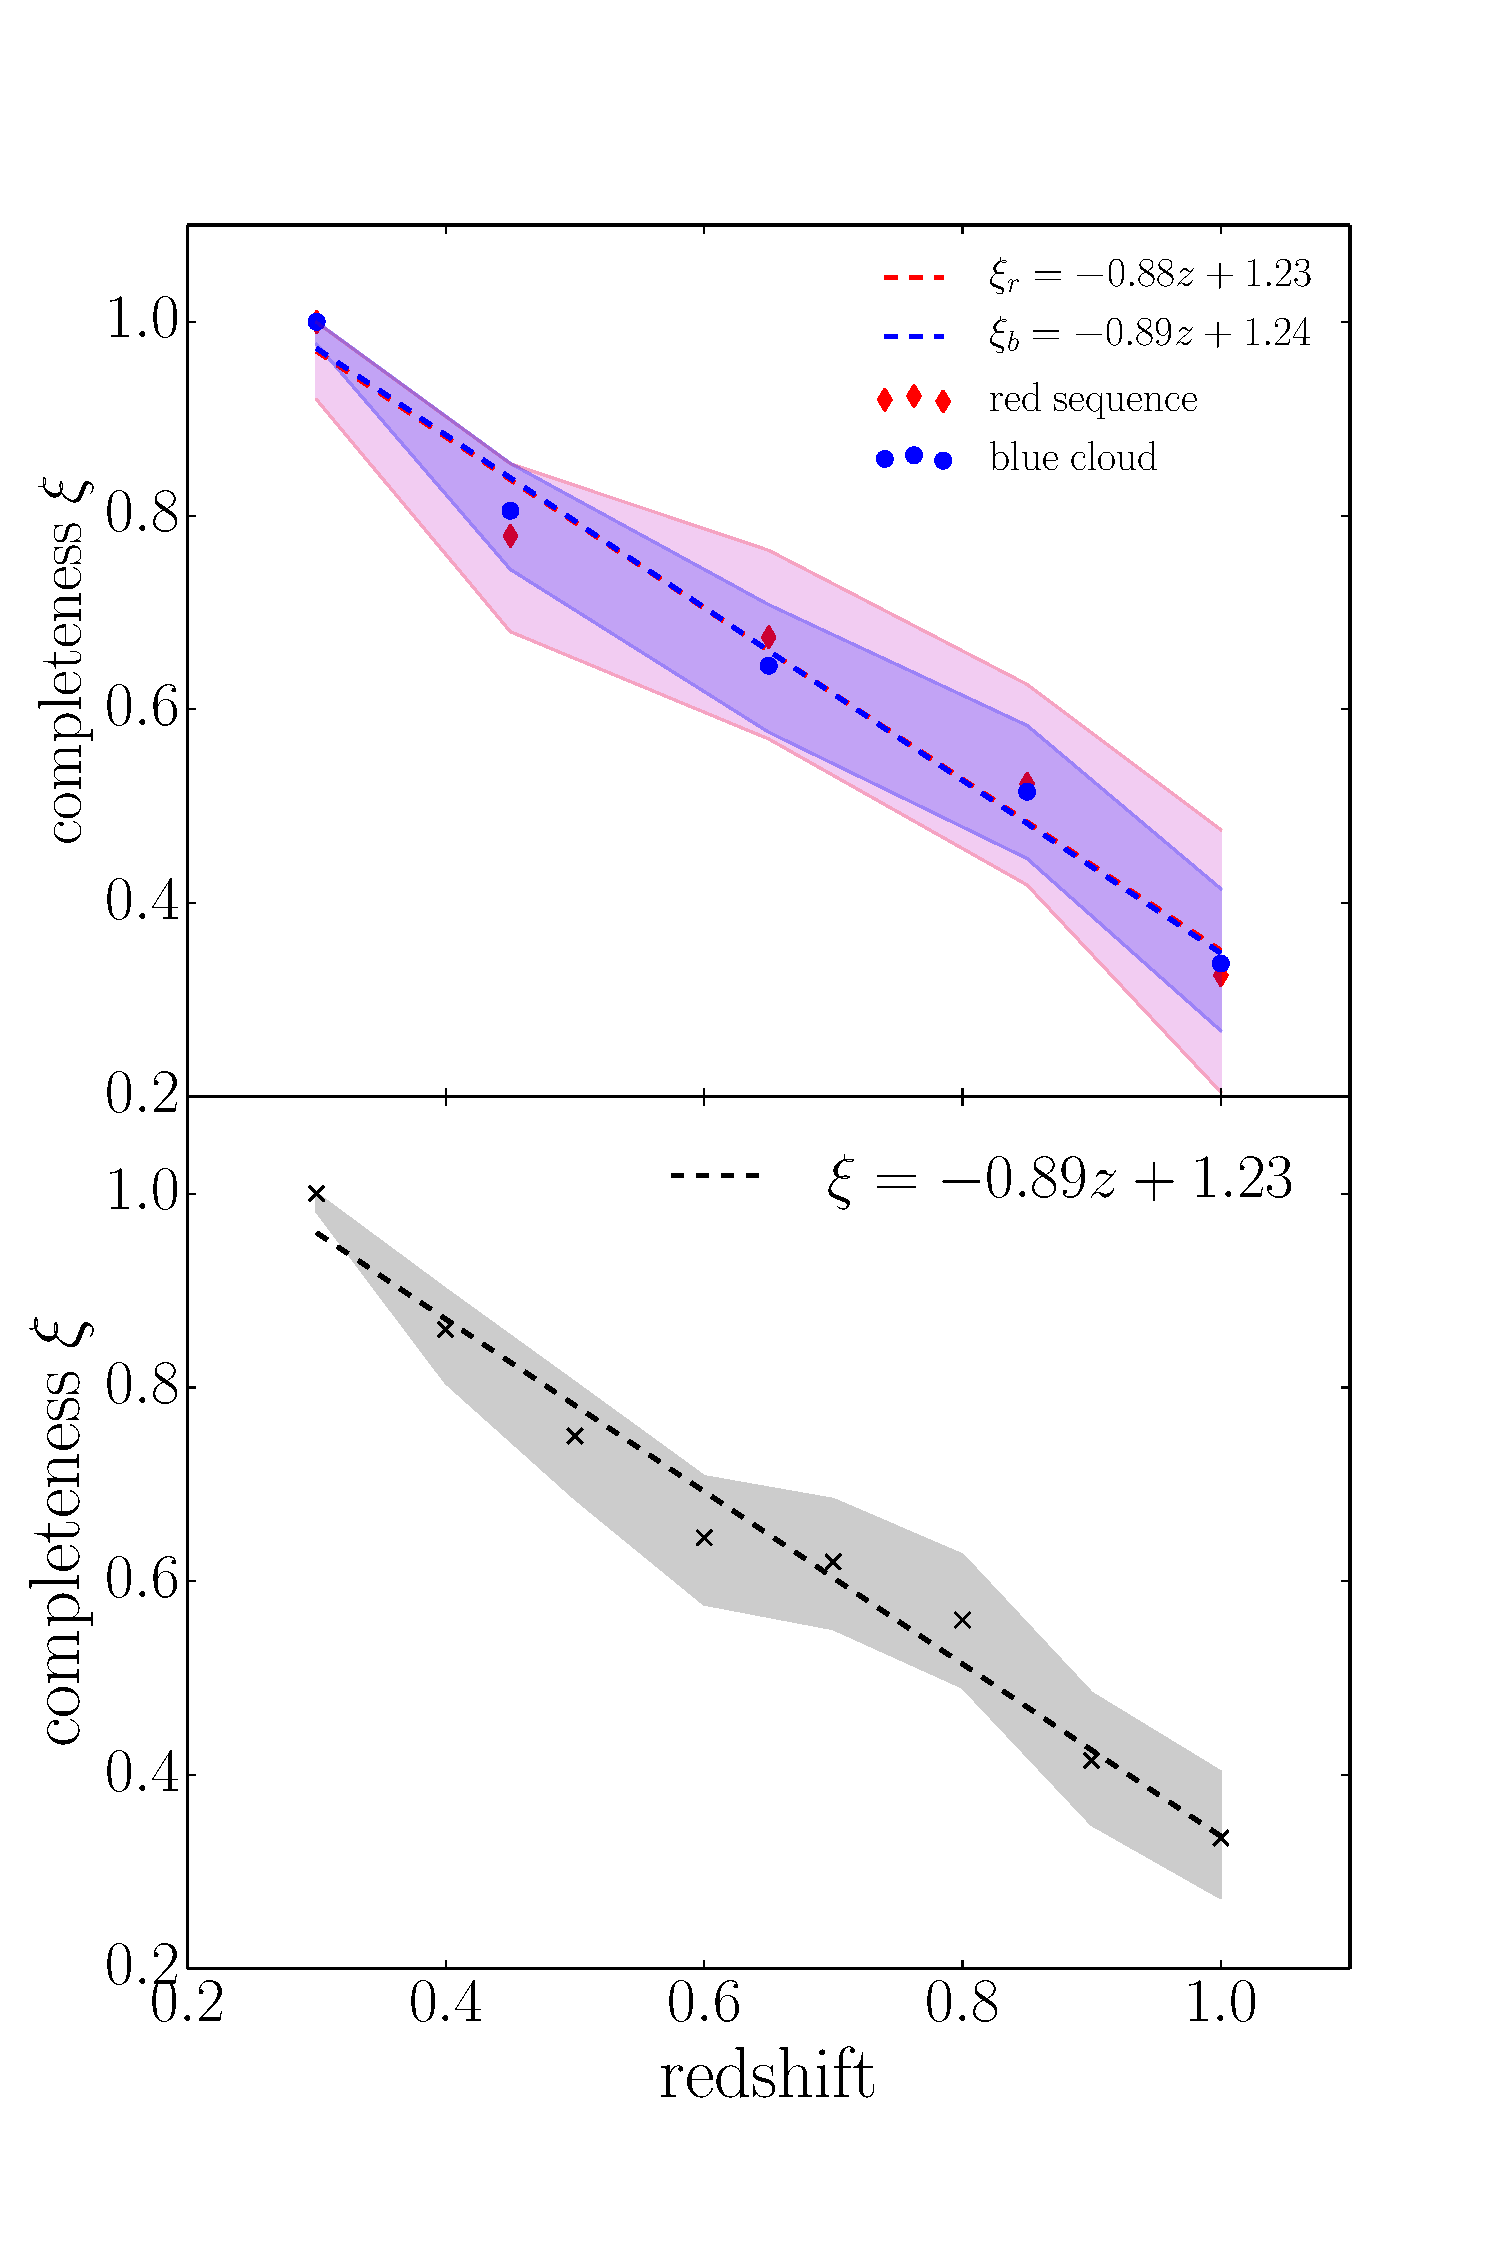
\includegraphics[width=3in,trim={0cm 2cm 2cm 1cm},clip]{figures/completenessmoneyplot.pdf}
\caption{\textbf{Top:} Completeness $\xi$ as a function of redshift for red sequence and blue cloud \ferengi2 galaxies separately. Both populations show a strong dependence on $\xi$ with redshift, but are indistinguishable from each other. \textbf{Bottom:} Completeness as a function of redshift for all  \ferengi2 galaxies (red and blue combined). The equation representing the linear fit is displayed.}
\label{fig:xi}
\end{figure}

\section{Results}
\label{sec:results}
In this section we present our results of the evolution of star-forming and quenched disc and elliptical galaxies from $z=1$ to $z=0.2$ in a sample of 2x,xxx $COSMOS$ galaxies morphologically classified in GZH. We show the evolution of each of the four types of populations as functions of redshift in four bins of stellar mass (Figure~\ref{fig:all_plot}), and the fractions of red disks galaxies with respect to all disks, and to all red sequence galaxies (Figure~\ref{fig:f_results}).

\begin{figure*}
\centering
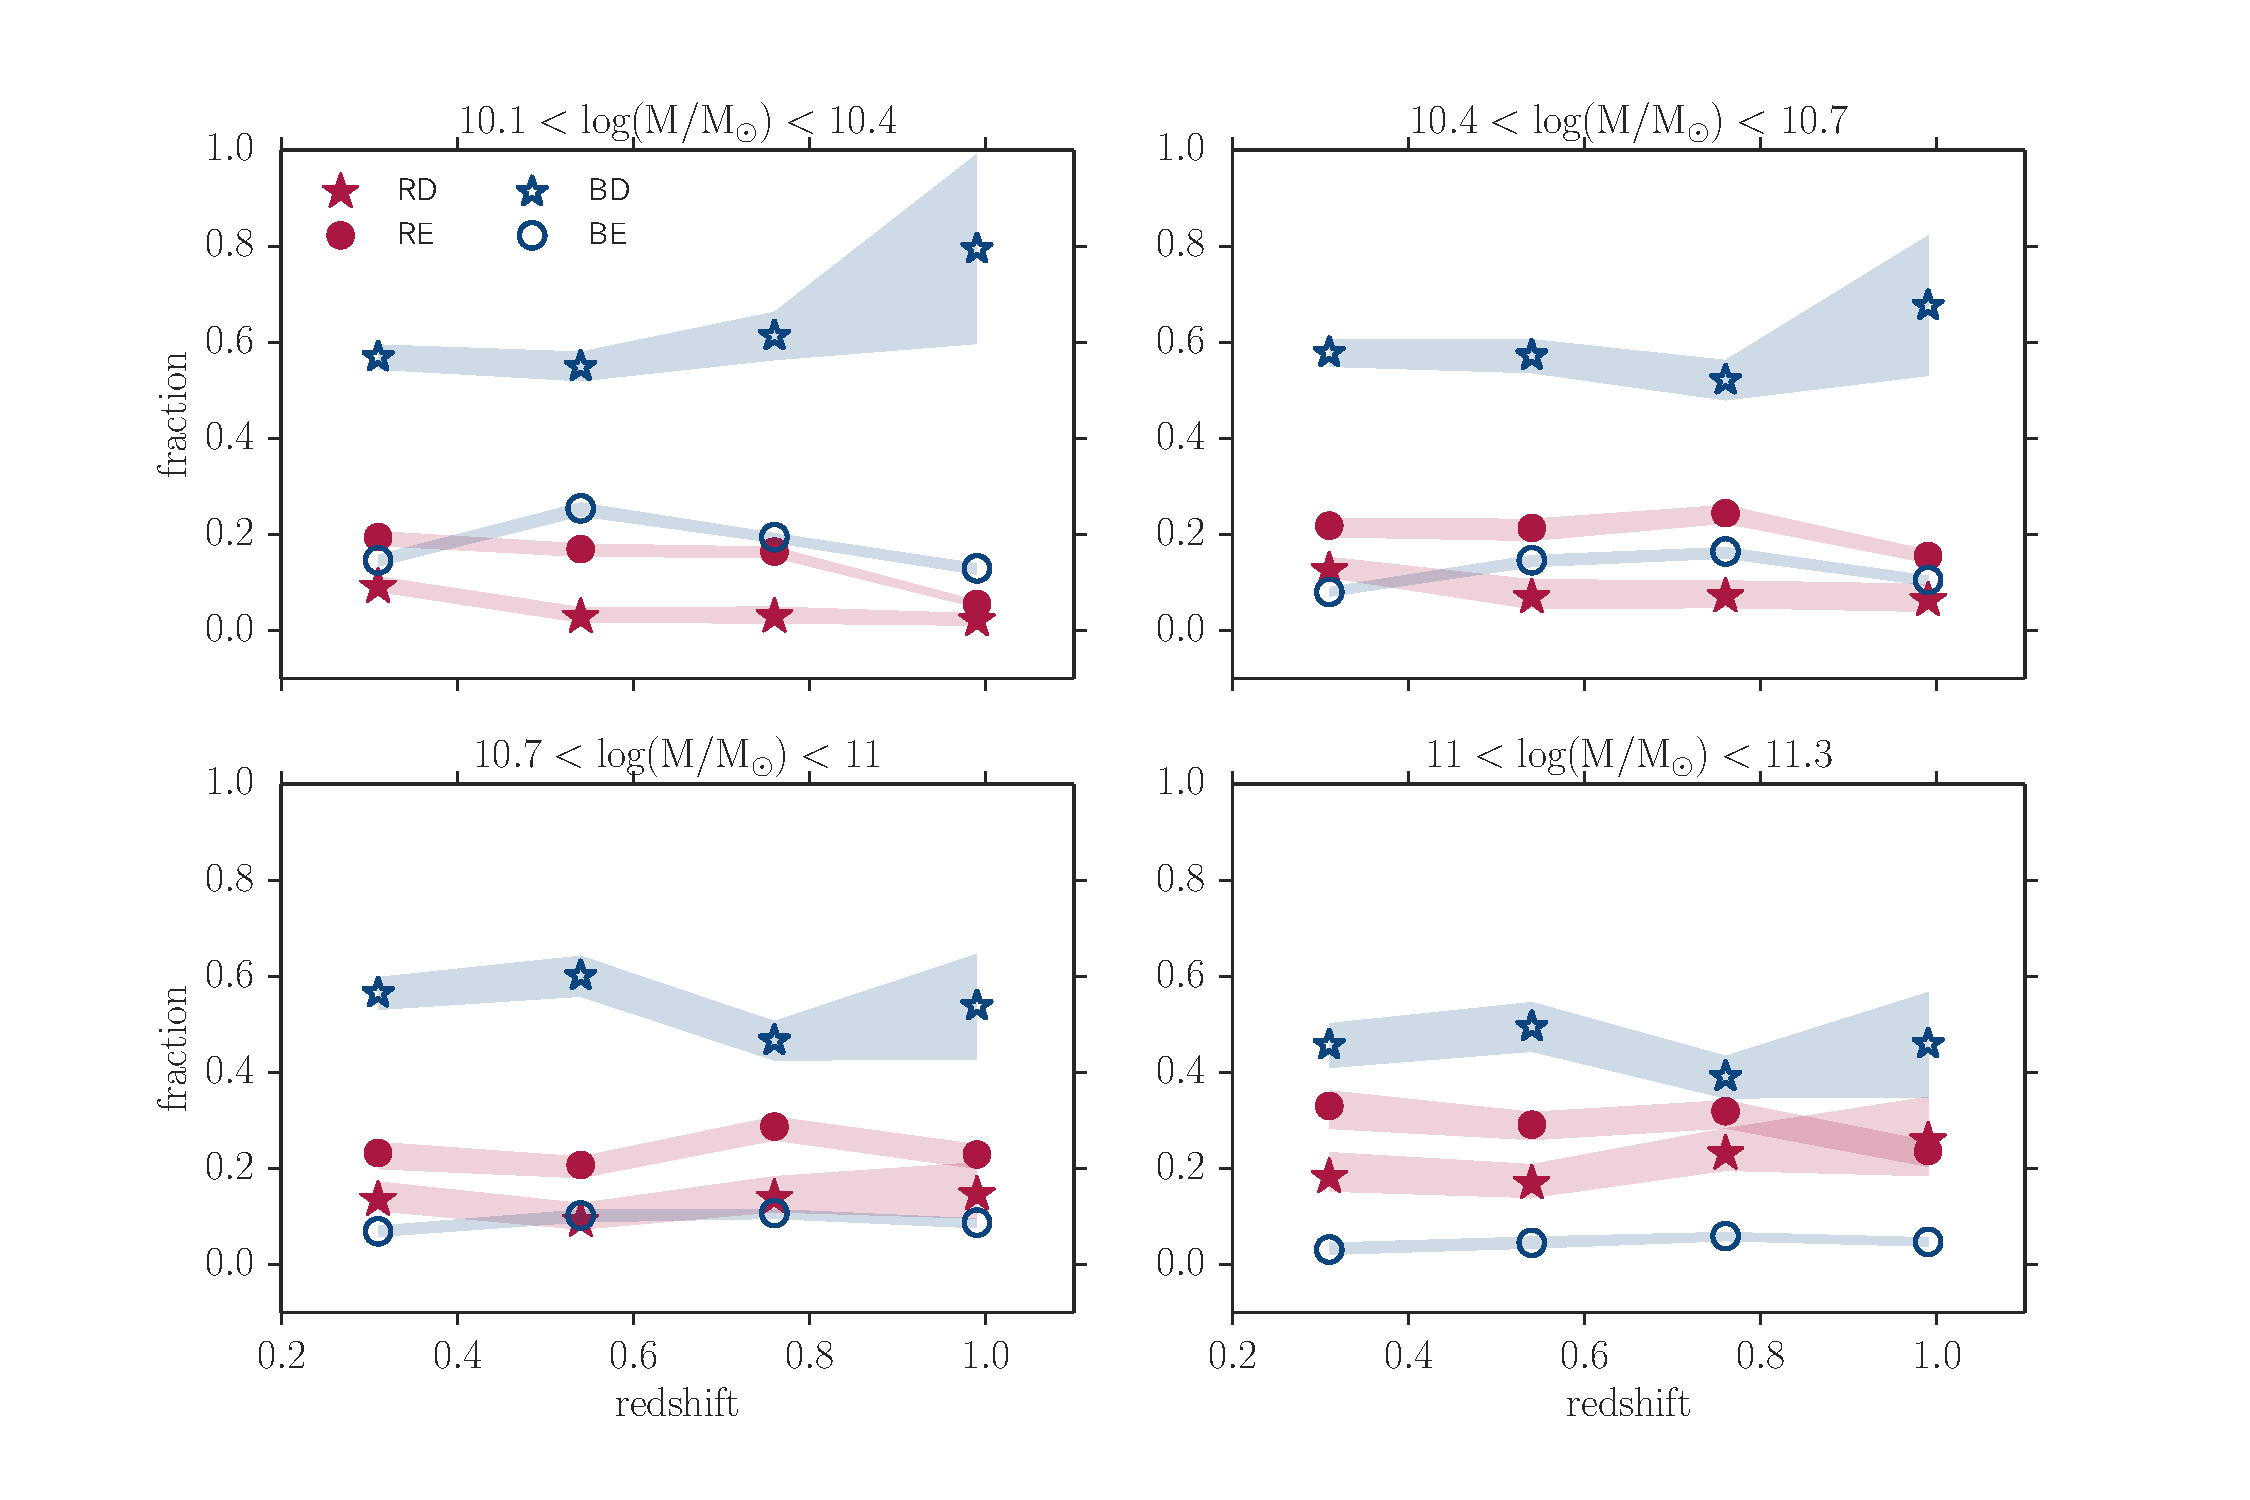
\includegraphics[width=\textwidth,trim={0cm 0cm 2cm 1cm},clip]{figures/morphologies_evolved.pdf}
\caption{Evolution of four types of galaxy populations since $z=1$: blue disks (blue open stars), red disks (red closed stars), blue ellipticals (blue open circles), and red ellipticals (red closed circles). Each point represents the fraction of the indicated type with respect to the total population, such that all points in a given redshift, mass bin sum to 1. Errors on each fraction are indicated by the shaded regions, and are propogations of $\sqrt{N}$ counting errors and the errors associated with the functional fits to the correction terms $\xi_{\rm disk}$ and $\xi_{\rm elliptical}$ (Section~\ref{ssec:xi}). }
\label{fig:all_plot}
\end{figure*}


\begin{figure*}
\centering
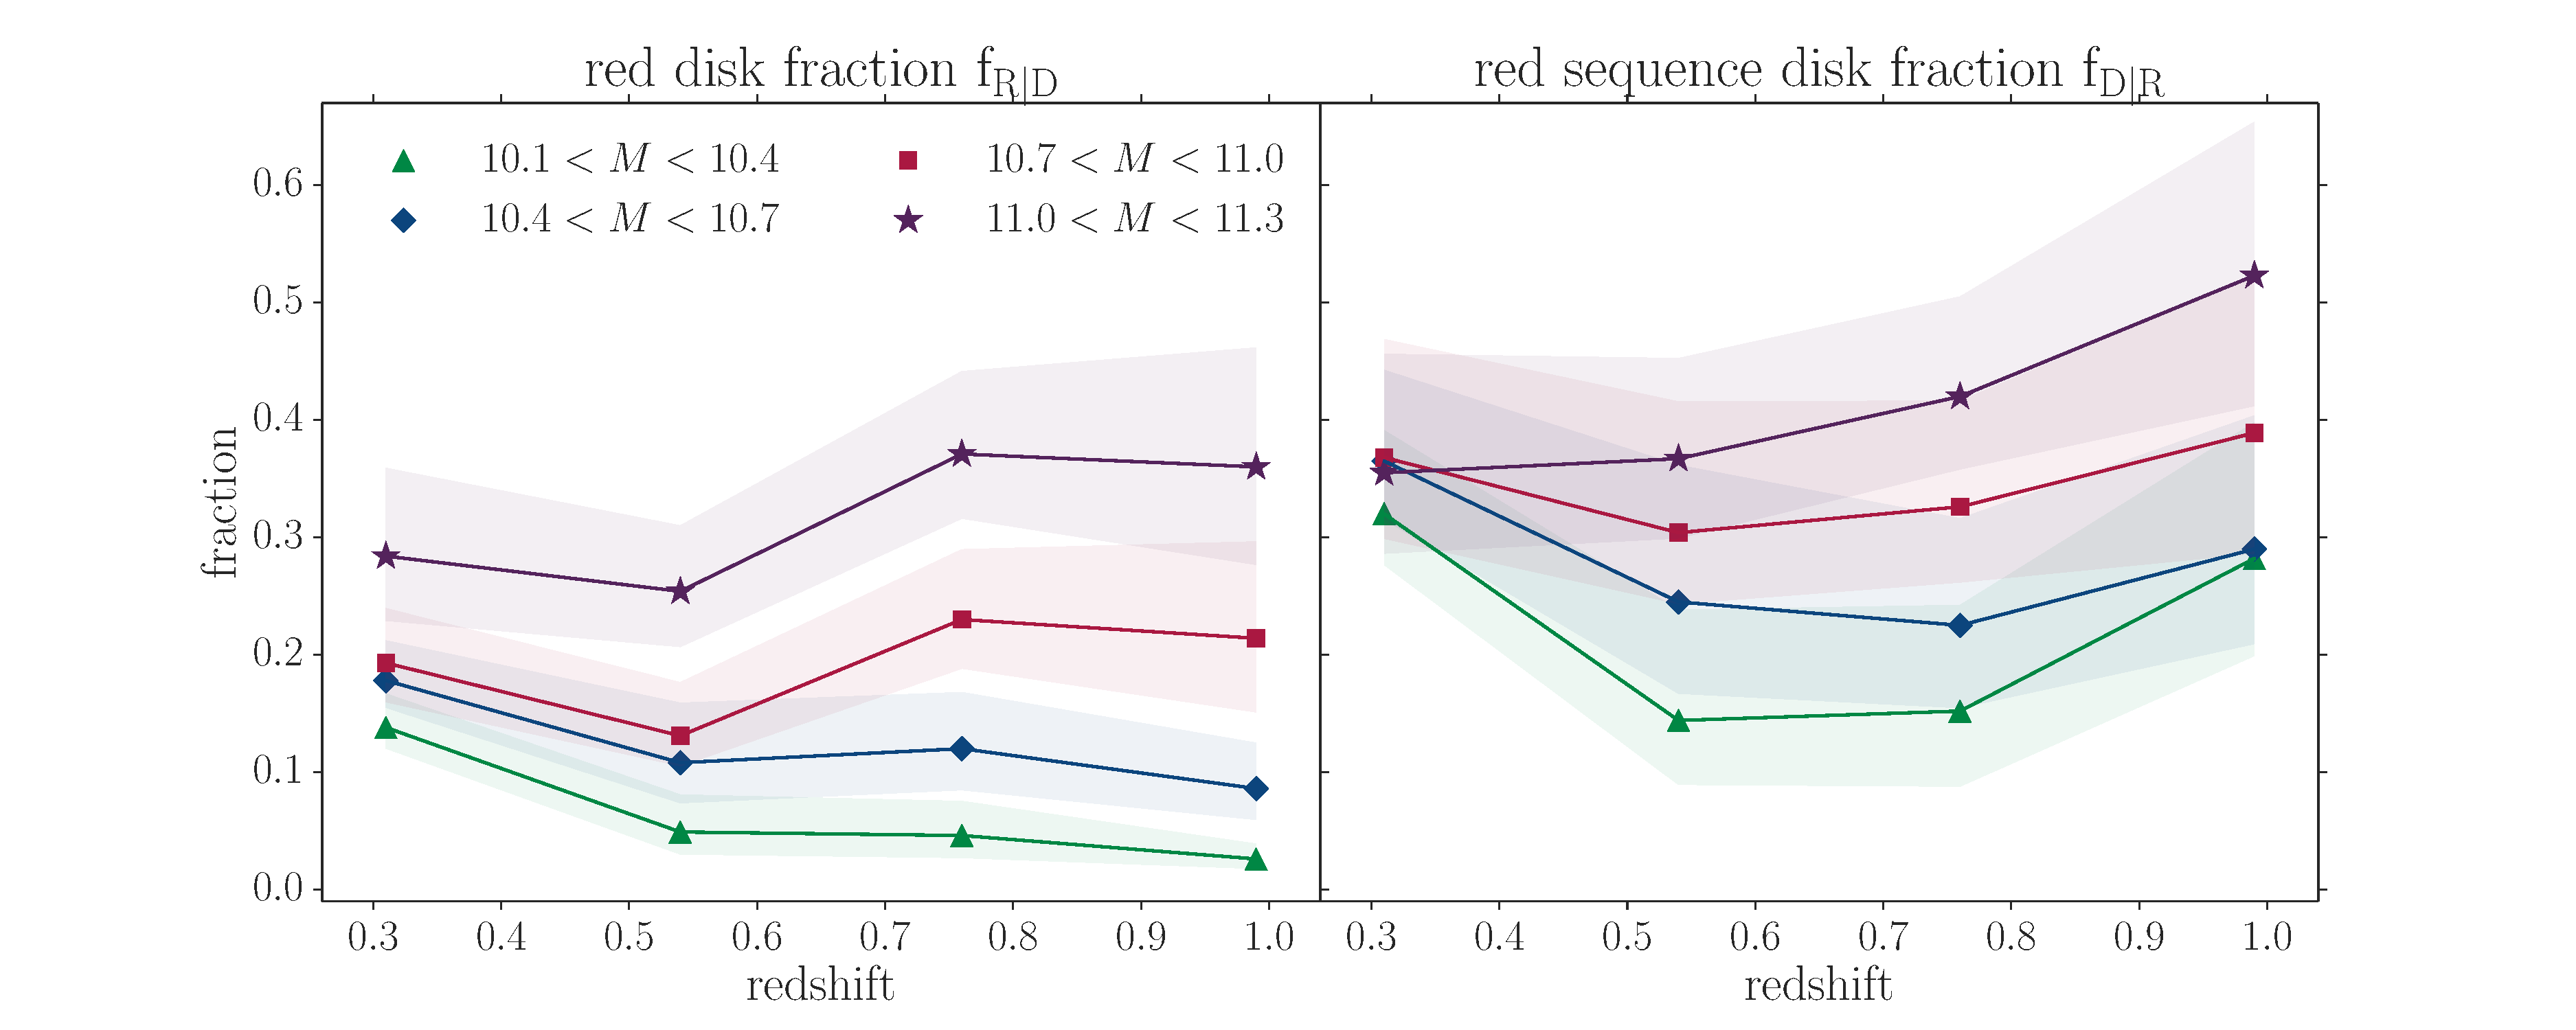
\includegraphics[width=\textwidth,trim={0cm 0cm 2cm 1cm},clip]{figures/red_disk_fractions.pdf}
\caption{\textbf{Left:} Passive disk fraction ($\rm N_{red~disks}/(N_{red~disks}+N_{blue~disks})$) vs redshift in four mass bins. \textbf{Right:} Fraction of disks on the red sequence ($\rm N_{red~disks}/(N_{red~disks}+N_{red~ellipticals})$) vs redshift in four mass bins. Errors on each fraction are indicated by the shaded regions, and are propogations of $\sqrt{N}$ counting errors and the errors associated with the functional fits to the correction terms $\xi_{\rm disk}$ and $\xi_{\rm elliptical}$ (Section~\ref{ssec:xi}).} 
\label{fig:f_results}
\end{figure*}


%super basic: absoluate numbers
In Figure~\ref{fig:all_plot} we plot the fractional contribution of blue/star-forming disks, blue/star-forming ellipticals, red/passive disks, and red/passive ellipticals vs. redshift in four stellar mass bins. For all masses, blue disks are the plurality population at each redshift. The red disk population is most abundant in the highest mass bin, and at fixed redshift their contribution decreases with mass. Red ellipticals tend to significantly outnumber red disks except in the highest mass/redshift bin, where they are in almost equal quantity. Blue ellipticals represent an insignificant fraction for galaxies with mass $\rm log(M/M_{\odot})>10.7$, but begin to outnumber the red disk population at lower masses. 

%next: trends
%explain SF?

%trends
Red disk galaxies are presumed to form primarily from blue disks galaxies which have quenched without undergoing a morphological transformation. If this is true, and if the resulting quenched disks do not continue in their evolution, one would expect a ``pile up'' of red disks as time progresses, resulting in an increasing fraction from right to left. This trend is observed in the two lowest mass bins, however there is no large change in fraction in the $M\sim10.85$ bin, and even a small decrease in the highest mass bin. If we assume that red disks are continuously produced from blue disks, even at a small rate, then a constant or decreasing fraction can only be explained if their numbers are simultaneously being depleted, presumably by a morphological transformation to red elliptical.

The evolution of the red disk population is more apparent in Figure~\ref{fig:f_results}. On the left is the ratio of red disks to all disks ($f_{\rm R|D} = \rm N_{\rm red~disks}/(N_{\rm red~disks}+N_{\rm blue~disks}))$, and the right shows the fraction of disks on the red sequence ( $f_{\rm D|R} = \rm N_{\rm red~disks}/(N_{\rm red~disks}+N_{\rm red~ellpticals}))$. In both fractions, there is a clear mass-dependence with the trends exhibited as functions of redshift. $f_{R|D}$ is constant for $M>10.7$, and increases for the lower mass bins. An increase in $f_{R|D}$ could be driven by the increase of red disks or a depletion of blue disks; Figure~\ref{fig:all_plot} shows the increase may be driven more from the latter at $z\sim1$, and the former at lower redshift. On the right, we find a decrease in $f_{D|R}$ for all masses in the interval from $z\sim1$ to $z\sim0.8$. Figure~\ref{fig:all_plot} shows that this is mainly driven by the increase in red ellipticals during this time, which is consistent with higher merger rates at this epoch (reference?). From $z\sim0.8$ to $z\sim0.3$, $f_{D|R}$ continues to decrease for galaxies $log(M/M_{\odot})>11$, is constant for galaxies $log(M/M_{\odot}\sim10.85$, and increases for the lower mass bins. From Figure~\ref{fig:all_plot}, we confirm that the increase present in the low mass galaxies is driven more by increases in the proportion of red disks, and not from a depletion of red ellipticals. The increase of $f_{R|D}$ and $f_{D|R}$ with redshift observed at low masses, coupled with the constant or decreasing trends for high masses, suggests that low mass red disk galaxies may be more likely to remain as such, while more massive red disk galaxies are more likely to further evolve via a morphological transformation. 

The downward trend we observe in $f_{D|R}$ for massive galaxies is in agreement with \citet{Bundy2010} (hereafter B10) who perform a similar analysis of the morphological makeup of the red sequence. As suggested previously, a downward trend of $f_{D|R}$ represents either a depletion of the total pool of red disks (via a transformation to elliptical), but could also be an indication of an increase in the pool of red ellipticals (which could result from blue or red disks transforming morphology). In contrast, an upward trend is only possible via a pile-up of red disks, which is what we observe for the lower mass bins, and is in disagreement with B10. At the lowest redshift bin ($z\sim0.3$), we measure similar absolute fractions of disks occupying the red sequence for all masses. However, B10 find their contribution to increase at higher lookback time to $z=1$, while we find a decreasing contribution. 

The fact that our results agree for the highest mass at all redshifts, but only at the lowest redshift for lower masses, suggests the differences may be attributed in biases in morphological classification. B10 identifies early and late-type disk galaxies using ZEST \citep{Scarlata2007} morphologies, which they acknowledge are biased towards disk classification for faint apparent magnitudes, which tend to be attributed to the lowest mass, highest redshift objects. This bias could influence their observed increase in red sequence disks toward $z=1$ for low masses. On the opposite end, GZ classifications tend to be biased towards elliptical morphologies at fainter magnitudes. We attempted to quantify and correct for this effect as described in Section~\ref{ssec:ferengi}, but if our correction was under-estimated, that may have driven the decreasing abundance of disk galaxies observed at increasing redshift for low masses. However, it has been shown in the local Universe that red disk galaxies tend to be more massive, as in \citet{Masters2011}. If this is true at all epochs, we would not expect such a significant contribution of red disks for low mass galaxies as found in B10.

\section{Discussion}
%first: reiterate what was done and with main conclusions/points drawn. 
We have examined the evolution of red disk galaxies since $z=1$ in Figures~\ref{fig:all_plot} and~\ref{fig:f_results}. The different trends observed in the abundance of red disks for different bins of mass are consistent with a physical scenerio in which 1) more massive galaxies undergo morphological transformations to elliptical at a higher rate than their less massive counterparts (given by the decrease/increase of $f_{D|R}$ from $z=1$ to $z=0.3$ for high/low mass bins), and 2) more massive galaxies are more likely to enter a red disk phase to begin with (given by the higher proportion of red disks in the high mass bin of Figure~\ref{fig:all_plot}). 

\begin{figure}
\centering
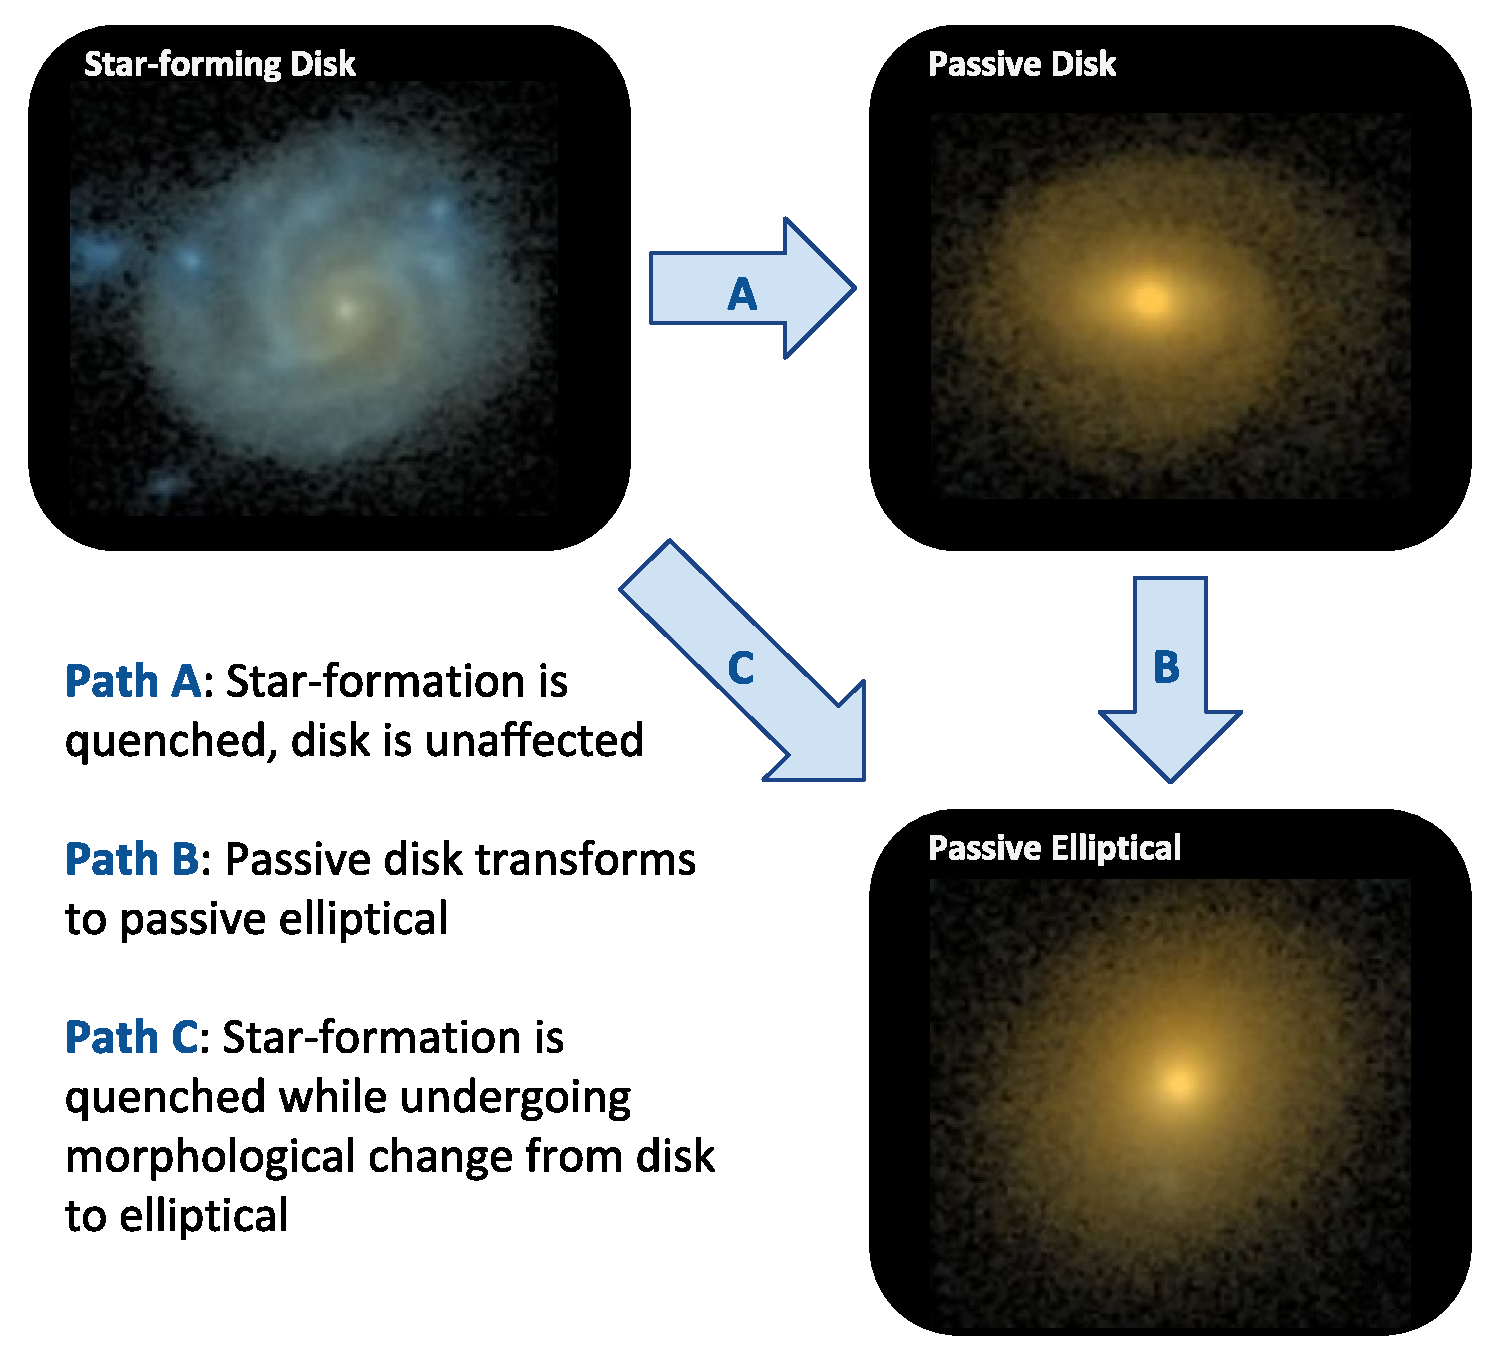
\includegraphics[width=3.5in]{figures/cartoon.pdf}
\caption{Cartoon representing three common evolutionary pathways of star-forming disk galaxies. Path A represents an active star-forming galaxy which quenches without destroying the disk, becoming a red disk. Path B represents a red disk morphologically transition to red ellipitcal. Path C represents a blue disks simultaniously quenching and morphologically transforming to become a red elliptical. }
\label{fig:cartoon}
\end{figure}

\subsection{Morphological transformation of red disks}

Our first point addresses whether the red disk form is a final stage in a galaxy's evolution, or whether it is a transitory phase in its ultimate path from star-forming disk to quenched elliptical. Figure~\ref{fig:cartoon} is a simple schematic of dominant quenching pathways for typical galaxies. If all galaxies adhered to the standard color-morphology relationship, we could conclude that all galaxies follow Path C: in this channel, whatever mechanism causes a galaxy to quench simultaneously invokes a morphological transformation. The existence of red disk galaxies insists that Path A is also a viable channel, in which a star-forming disk quenches without any significant structural disruption. If these were the only two channels, we would expect pile ups of red disks as the Universe evolves. We observe such pile ups for low-mass red disk galaxies, but not for more massive galaxies; this suggests that Path B, the depletion of red disks via a later morphological transformation, is necessary to deplete the pool and counteract the pile up effect.

It has been long suggested that major-mergers are the dominant mechanism for transforming the majority disk-like galaxies to elliptical \citep{Toomre1977,Schweizer1982,Schweizer1990}, with multiple minor-mergers being the second-most dominant~\citep{Bundy2009,Hopkins2010b}. Studies using observations of close pairs have shown the galaxy merger rate increases with mass, both in the local Universe \citep{Xu2004,Patton2008,Domingue2009,Robotham2014,Casteels2014} and out to $z\sim1$ \citep{Xu2012,Bundy2009}, which agrees with predictions from both empirical models and dynamical simulations \citep{Hopkins2010a,Hopkins2010b,Maller2006}. \citet{Casteels2014} find the merger rate is as much as three times higher for massive ($\rm log(M/M_{\odot})\sim11.25$) than lower mass ($\rm log(M/M_{\odot})\sim8.25$) galaxies, a similar mass range probed in our study. The increasing merger rate with mass may explain why massive red disk galaxies do not tend to stay in this phase long before merging, while low mass galaxies which become red disks remain stable in that phase. 


\subsection{The formation of red disks}

Our results suggest that red disks represent a prolonged or final stage in the evolution of low mass galaxies, while high mass red disks are unlikely to remain in such a phase, due to an increased merger rate for higher mass galaxies. Next we address our second point: what mechanisms can cause a galaxy to quench without transforming morphologically (Path A, Figure~\ref{fig:cartoon}), and why is this channel more common in massive galaxies? 
 
\subsubsection{Secular quenching of blue disks}

Perhaps the most straight-forward mechanism by which a disk could quench without changing morphology is a purely secular process, in which an isolated galaxy's gas supply is simply used up from continued star-formation. It is rare, however, for a galaxy to exist in complete isolation long enough for this scenario to occur. The time-scale for complete consumption of gas with no environmental disruptions can be estimated from the amount of gas in a typical galaxy and the rate it is consumed through star-formation: $\tau \sim M_{gas}/{M}_{gas}$, typical estimates giving several Gyr for total depletion \citep{Larson1980,Kaviraj2011,Hatton2003,Schawinski2014}. Most galaxies will have experience some kind of environmental interaction within this time [need to find reference of average interaction time / average number of mergers for this argument to hold.]. [this source] suggests this many galaxies experience this many mergers in this time. Further, the fraction of galaxies in the field is quite low - \citet{Tully1987} find the fraction of true isolated galaxies is less than 1\% in the local Universe. 

Since environmental interactions tend to impact the morphology of a galaxy, a simple check would be a comparison of features of disks in the red sequence and blue cloud. B10 using the ZEST classification scheme find the bulk of red sequence disks are early-type, while the late-type disks are found primarily in the blue cloud. The Galaxy Zoo classifications do not offer a comparable method for distinguishing late and early type galaxies, but we can use the bulge prominence information as a proxy. We note that a complete analysis of bulge prominence cannot be done here, as there has been no proper redshift debiasing of this vote fraction, and a thorough investigation will be saved for future work. As a preliminary check, we compare the bulge prominence of red sequence and blue cloud disk galaxies for a low-redshift ($z<0.4$) sample, where any biases should be minimal. 

In GZH, users who have classified a galaxy as featured and not edge-on are instructed to vote on the prominence of the bulge by choosing one of four responses: ``no bulge,'' ``just noticeable'', ``obvious'', and ``dominant''. For this analysis we will compare the sum of the vote fractions $f_{\rm obvious} + f_{\rm dominant}$ for red sequence and blue cloud disk galaxies, shown in Figure~\ref{fig:bulge}. We find a clear difference in distributions, such that the red sequence disks tend to have more prominant bulges. While we present the results of the $z<0.4$ sample to minimize potential redshift bias, we note that the result holds when extended to all redshifts. This supports the conclusions of B10, given that early-type classifications are correlated with dominant bulges. This also agrees with \citet{Masters2010}, who also find larger bulge prominences in red sequence disks for a local Universe sample using Galaxy Zoo 2 classifications.

Given the timescales required for pure secular quenching, compared with the typical merger rate and the low average number of field galaxies, and the apparent morphological differences between the blue cloud and red disk population, it seems unlikely that this option contributes to a significant portion of the red disk population.  

\begin{figure}
\centering
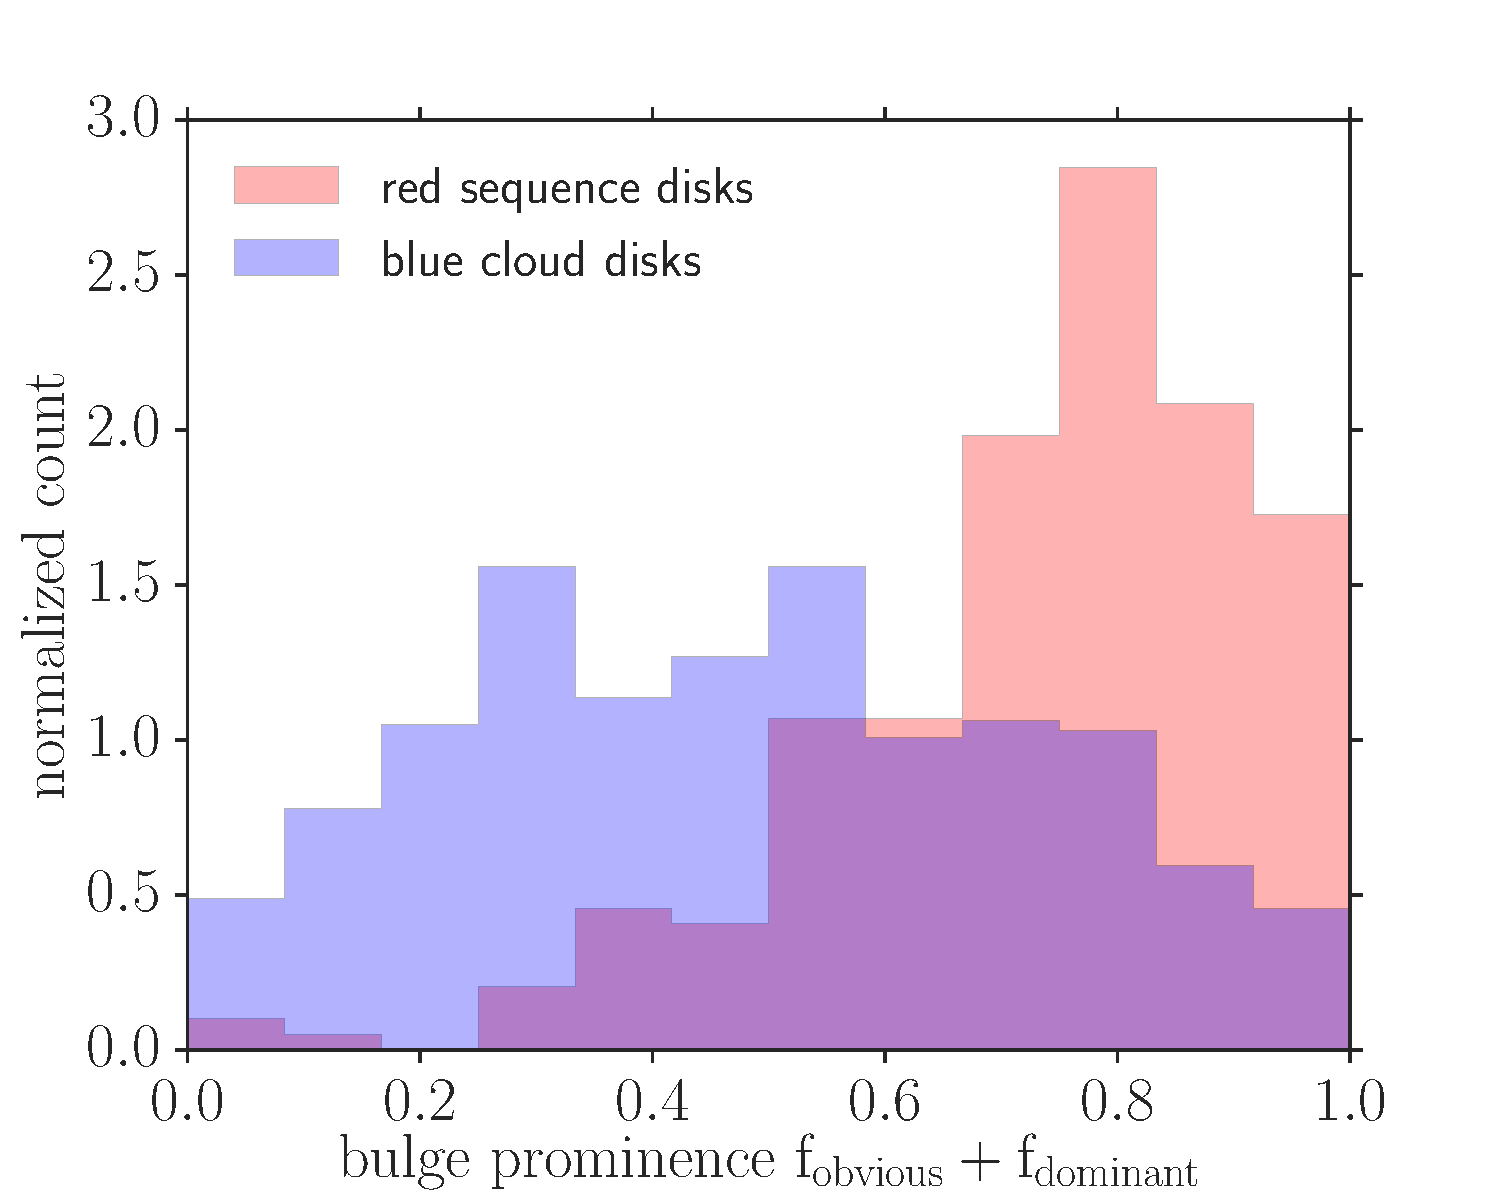
\includegraphics[width=3.5in]{figures/bulge_comparison.pdf}
\caption{Comparison of bulge prominence of blue cloud disks and red sequence disks, using GZH vote fraction $f_{\rm obvious} + f_{\rm dominant}$ as indicator of the observed relative size of the bulge. Only galaxies $z<0.4$ are shown to minimize potential effects of redshift bias in these vote fractions, which have not been corrected for in this paper (although the result does hold out to $z\sim1$). Red disks tend to have more prominent bulges than blue cloud disks, and almost zero red sequence disks have extremely low bulge prominences ($f_{\rm obvious} + f _{\rm dominant} < 0.3$).}
\label{fig:bulge}
\end{figure}
  
\subsubsection{Mass quenching and AGN feedback}
In some cases the mass of a galaxy might cause (rather than correlate with) the formation of a red disk, via mass quenching \citep{Kormendy2004,Peng2010,Schawinski2014,Smethurst2017}. For most galaxies, star-formation is enabled via cold streams of accreting gas \citet{Dekel2006}. Simulations \citep{Birnboim2003,Cattaneo2006} show that as a galaxy halo reaches a critical mass $M_{halo}>10^{12}M_{\odot}$, virial shocks heat the gas, resulting in a cutoff of the galaxy's gas reservoir, inhibiting star-formation. 

Dilution of gas in massive galaxies due to such shock-induced heating can cause it to become more vulnerable to AGN feedback \citep{Dekel2006}, wherby accretion onto the galaxy's supermassive black hole generates strong outflows of energetic material and hard radiation. These AGN-driven winds may then terminate star-formation by heating the gas or expelling it completely from the galaxy, causing a quench. Such a process is not likely to induce a morphological transformation, and therefore could be a valid mechanism for creating a quenched disk. This effect was first proposed in an effort to accurately model the local-Universe luminosity function. Only models which incorporated AGN feedback to supress star-formation in the most massive galaxies could reproduce the sharp break observed in the number density of highly luminous galaxies \citep{Benson2003,DiMatteo2005,Bower2006,Croton2006,Somerville2008}. \citet{Smethurst2016} found strong evidence for rapid and recent quenching through an analysis of star formation histories of a large population of AGN hosts. Although they did not explore whether this effect was mass-dependent, it nevertheless suggests AGN-feedback does play a strong role in the quenching of galaxies. Furhter, since AGN tend to be observed in more massive galaxies \citep{Schawinski2007,Lee2012,Oh2012,Alonso2013,Galloway2015}, it is reasonable to suggest AGN-induced quenching may be a significant contributor to the formation of massive red disks. 

\subsubsection{Disk regrowth in mergers}

It is believed that ellipticals are the products of mergers, however recent evidence has shown that mergers do not always produce ellipticals. Simulations have shown cases of rotationally supported disks surviving or reforming after a major merger event. This tends to be possible under conditions such that the projenitor disks are gas-dominated \citep{Governato2009,Springel2005a}; for \citet{Robertson2006} disks were only formed if the gas-fractions exceeded $f_{gas}>0.5$. Under these conditions, it would be more likely to form low-mass disks, given that gas fraction tends to anti-correlated with stellar mass \citep{Kannappan2004,Bell2000}. Perhaps this mechanism could explain some portion of the low-mass red disk population. However, regrown disks in these simulations tend to arise as star-forming. If the merger-disk regrowth event enhances star-formation briefly, perhaps the remaining gas is used up in a shorter time-scale, leading to a low-mass red disk. \citet{Sparre2017} find that although most of the new disks were star-forming, some were immediately quenched in the simulations which incorporated particularly strong AGN feedback. Since AGN are found more commonly in high mass galaxies, this scenario could account for some fraction of the high-mass red disk population.

\subsection{Looking forward: developing a model to reproduce observations}

Through observations of the evolution of the red disk popluation since $z=1$, we have deduced that massive galaxies are more likely to both enter a red disk phase and subsequently exit the stage via a morphological transformation, while low mass disks which enter a passive stage are more likely to remain in that phase than continue their evolution. To quantify and verify this interpretation would require further work, such as a semi-analytical model which could reproduce these observations given parameters describing the rate of occurances of the different evolutionary pathways shown in Figure~\ref{fig:cartoon}. A complete model is beyond the scope of this work, but an example of a simple toy-model approach is given in the appendix. Our simple model was not able to constrain values for all parameters implemented, but it did detect a mass-dependene on the rate at which blue disks transform to red disks, which agrees with our interpretations thus far. 

\section{Conclusions}
\label{sec:conclusions}

We have investigated the influence of the passive disk population by measuring the relative abundances of blue disks, red disks, blue ellipticals, and red ellipticals since $z=1$ using morphological classifications from Galaxy Zoo: Hubble and rest-frame colors from UltraVISTA. Using data from artificially-redshifted \ferengi2 images to quantify the known redshift bias in the GZ classifications, we implemented a correction to the incompleteness in the number of disks and ellipticals detected as a function of redshift. The relative numbers were measured in terms of the fraction of disk galaxies that are red $f_{R|D}$ and the fraction of disk galaxies on the red sequence $f_{D|R}$. Our main conclusions are as follows:

\begin{itemize}

\item{$f_{R|D}$ and $f_{D|R}$ decrease from $z=1$ to $z=0.3$ for massive galaxies, and increase for the least massive galaxies.}

\item{Low mass galaxies which experience a passive disk phase are more likely than massive galaxies to remain disks, while massive galaxies are more likely to continue thier evolution by transforming to passive ellipticals. To quantify and validate this result would require a the implementation of a semi-analyitic model.}


\end{itemize}





%%%%%%%%%%%%
%%% ACKNOWLEDGMENTS
%%%%%%%%%%%%
The data in this paper are the result of the efforts of the Galaxy~Zoo~Hubble volunteers, without whom none of this work would be possible. Their efforts are individually acknowledged at \url{authors.galaxyzoo.org}. Please contact the author(s) to request access to research materials discussed in this paper. 


MG, CS, MB, and LF gratefully acknowledge support from the US National
Science Foundation Grant AST1413610.

This publication makes use of data products from the Two Micron All Sky Survey, which is a joint project of the University of Massachusetts and the Infrared Processing and Analysis Center/California Institute of Technology, funded by the National Aeronautics and Space Administration and the National Science Foundation.

This project made heavy use of the Astropy packages in Python \citep{Robitaille2013}, the \texttt{seaborn} plotting package \citep{Waskom}, and the Tool for OPerations on Catalogues And Tables (TOPCAT), which can be found at \url{www.starlink.ac.uk/topcat/} \citep{Taylor2005}. 

Funding for the SDSS and SDSS-II has been provided by the Alfred P. Sloan
Foundation, the Participating Institutions, the National Science Foundation,
the U.S. Department of Energy, the National Aeronautics and Space
Administration, the Japanese Monbukagakusho, the Max Planck Society, and the
Higher Education Funding Council for England. The SDSS website is
\url{http://www.sdss.org/}. 

The SDSS is managed by the Astrophysical Research Consortium for the
Participating Institutions. The Participating Institutions are the American
Museum of Natural History, Astrophysical Institute Potsdam, University of
Basel, University of Cambridge, Case Western Reserve University, University of
Chicago, Drexel University, Fermilab, the Institute for Advanced Study, the
Japan Participation Group, Johns Hopkins University, the Joint Institute for
Nuclear Astrophysics, the Kavli Institute for Particle Astrophysics and
Cosmology, the Korean Scientist Group, the Chinese Academy of Sciences
(LAMOST), Los Alamos National Laboratory, the Max-Planck-Institute for
Astronomy (MPIA), the Max-Planck-Institute for Astrophysics (MPA), New Mexico
State University, Ohio State University, University of Pittsburgh, University
of Portsmouth, Princeton University, the United States Naval Observatory and
the University of Washington. 

\bibliographystyle{mn2e}
\bibliography{/home/mel/Documents/Papers/library}  


\newpage
\clearpage

\appendix

\section{Toy-model approach to constrain rates of different evolutionary pathways}

Our observations of the fractional evolution of different morphological and activity types of galaxies since $z=1$ are well-suited for the implementation of a model to constrain the frequencies of different evolutionary pathways. Here we present our preliminary attempt at a toy model used to reproduce our observations, given different sets of input parameters. This is intended to be a suggested starting point for the further development of a sophisticated, semi-analytic model to describe and constrain potential rates of quenching and morphological evolution. 

We implement a simple toy model to track the change in $f_{R|D}$ and $f_{D|R}$, given a range of parameters representing the quenching and morphological transformation rates for galaxies at fixed stellar mass. We begin by considering the rate of change in the number of blue disks ($dN_{BD}/dt$), red disks ($dN_{RD}/dt$), and red ellipticals ($dN_{RE}/dt$). In a given mass bin, the change in numbers for each population will depend on several parameters, illustrated visually in Figure~\ref{fig:cartoon}.

\subsubsection{Blue Disks}
First, galaxies in a blue bin may transition into a red disk bin via a quenching process that does not destroy its disk; we define this rate as $r_{BD \rightarrow RD}$, representing the fraction of blue galaxies to transition to red disks per Gyr (path A in Figure~\ref{fig:cartoon}). Blue galaxies may also exit a bin via a quenching process which \emph{does} destroy the disk; this fraction per Gyr we define as $r_{BD \rightarrow RE}$ (path C in Figure~\ref{fig:cartoon}).

The number of galaxies in a blue disk bin will also change due to star formation, which brings active galaxies from a lower mass bin into the current mass bin. To account for this term we use the formalism outlined by \citet{Peng2010}, in which this rate of change is given by $(\alpha + \beta)sSFR$. Here $\alpha = d\phi_{blue}/dm$ is the derivative of the mass function for blue galaxies, which equates to $\alpha = (1+\alpha_s) - m/M^*$ for a mass function described by the Schechter (1976) function. We use best-fit parameters for blue galaxies measured by Johnpaperetal, which give $\alpha_s = -1.4$ and $M^* = 10.28 ~(log(M/M_{\odot}))$. Following the method of \citet{Peng2010}, we let $\beta=0$, both for simplicity, and because their conclusions found not to be strongly dependent on $\beta$. Last, the specific star-formation rate is given by $sSFR(t) = 2.5(\frac{t}{3.5 Gyr})^{-2.2}Gyr^{-1}$ \citep{Peng2010}.

Accounting for all sources and sinks of blue disks entering or exiting a bin of given mass, the rate of change of blue disks can be written fully as:

\begin{equation}
\frac{dN_{BD}}{dt}\Big\rvert_{m} = \Big(-r_{BD \rightarrow RD} - r_{BD\rightarrow RE} -\alpha(m) sSFR(t) \Big)N_{BD}
\label{eqn:BD}
\end{equation}

\subsubsection{Red Disks}
Galaxies exiting a blue bin as they quenched without disrupting their disks enter the pool of red disks, increasing $N_{RD}$ for a given mass bin. Red disks also may undergo a morphological transformation, depleting the pool of red disks as they enter the red elliptical bin (path B in Figure~\ref{fig:cartoon}). The fraction of galaxies to undergo this pathway per Gyr is denoted as $r_{RD->RE}$. Combining these factors gives the expression: 

\begin{equation}
\frac{dN_{RD}}{dt}\Big\rvert_{m} = + r_{BD \rightarrow RD}N_{BD} - r_{RD \rightarrow RE}N_{RD}
\label{eqn:RD}
\end{equation}

\subsubsection{Red Ellipticals}
In this simple model, it is assumed that red, passive ellipticals are the final state in a typical galaxy's evolution. Therefore $N_{RE}$ will always be increasing from the transformation from blue disks and red disks to red ellipticals ($r_{BD \rightarrow RE}$, $r_{RD \rightarrow RE}$). However, the number of red ellipticals \emph{in a single mass bin} may still decrease due to ellipticals at the given mass merging to enter a bin of red ellipticals at a higher mass. Similarly, their number can increase as ellipticals from a lower mass bin merge to enter the current mass bin. A complete, semi-analytic model would consider this full range of possibilities and couple the resulting equations appropriately amongst all mass bins. For the purposes of this simple model, we opted to represent the total, net rate of change of the number of red ellipticals as a single parameter, $\kappa_{RE}$, which we note may be positive or negative, depending on whether more ellipticals are entering or leaving the given mass bin. 

\begin{equation}
\frac{dN_{RE}}{dt}\Big\rvert_{m} = \kappa_{RE} N_{RE}  
\label{eqn:RE}
\end{equation}

We exclude the contribution from blue ellipticals from the model for maximum simplicity, and because they represent only a small fraction of the total population at most masses. A complete version of the model would include this population. We initialize our model using the observed relative numbers of blue disks, red disks, and red ellipticals measured at $z=1$, then use the model to compute their evolution to $z=0.3$ using a range of values for each of the four parameters in four mass bins. For $r_{BD \rightarrow RD}, r_{BD \rightarrow RE},$ and $r_{RD \rightarrow RE}$, we test 25 values between 0 and 1, and 25 values between -1 and 1 for $\kappa_{RE}$. We note that a complete model would explore time-varying rates, but for the purposes of simplicity in our toy-model we only experiment with static parameters. For each mass bin, the model was implemented for each permutation of the four rate parameters. The success of each run was evaluated using a $\chi^2$ metric; these results are shown for each mass bin in the corner-plot in Figure~\ref{fig:corner}. The bins are weighted by $1/\chi^2$, such that white regions represent the rate parameters that yield the lowest $\chi^2$, and black representing the largest.

\begin{figure*}
\centering
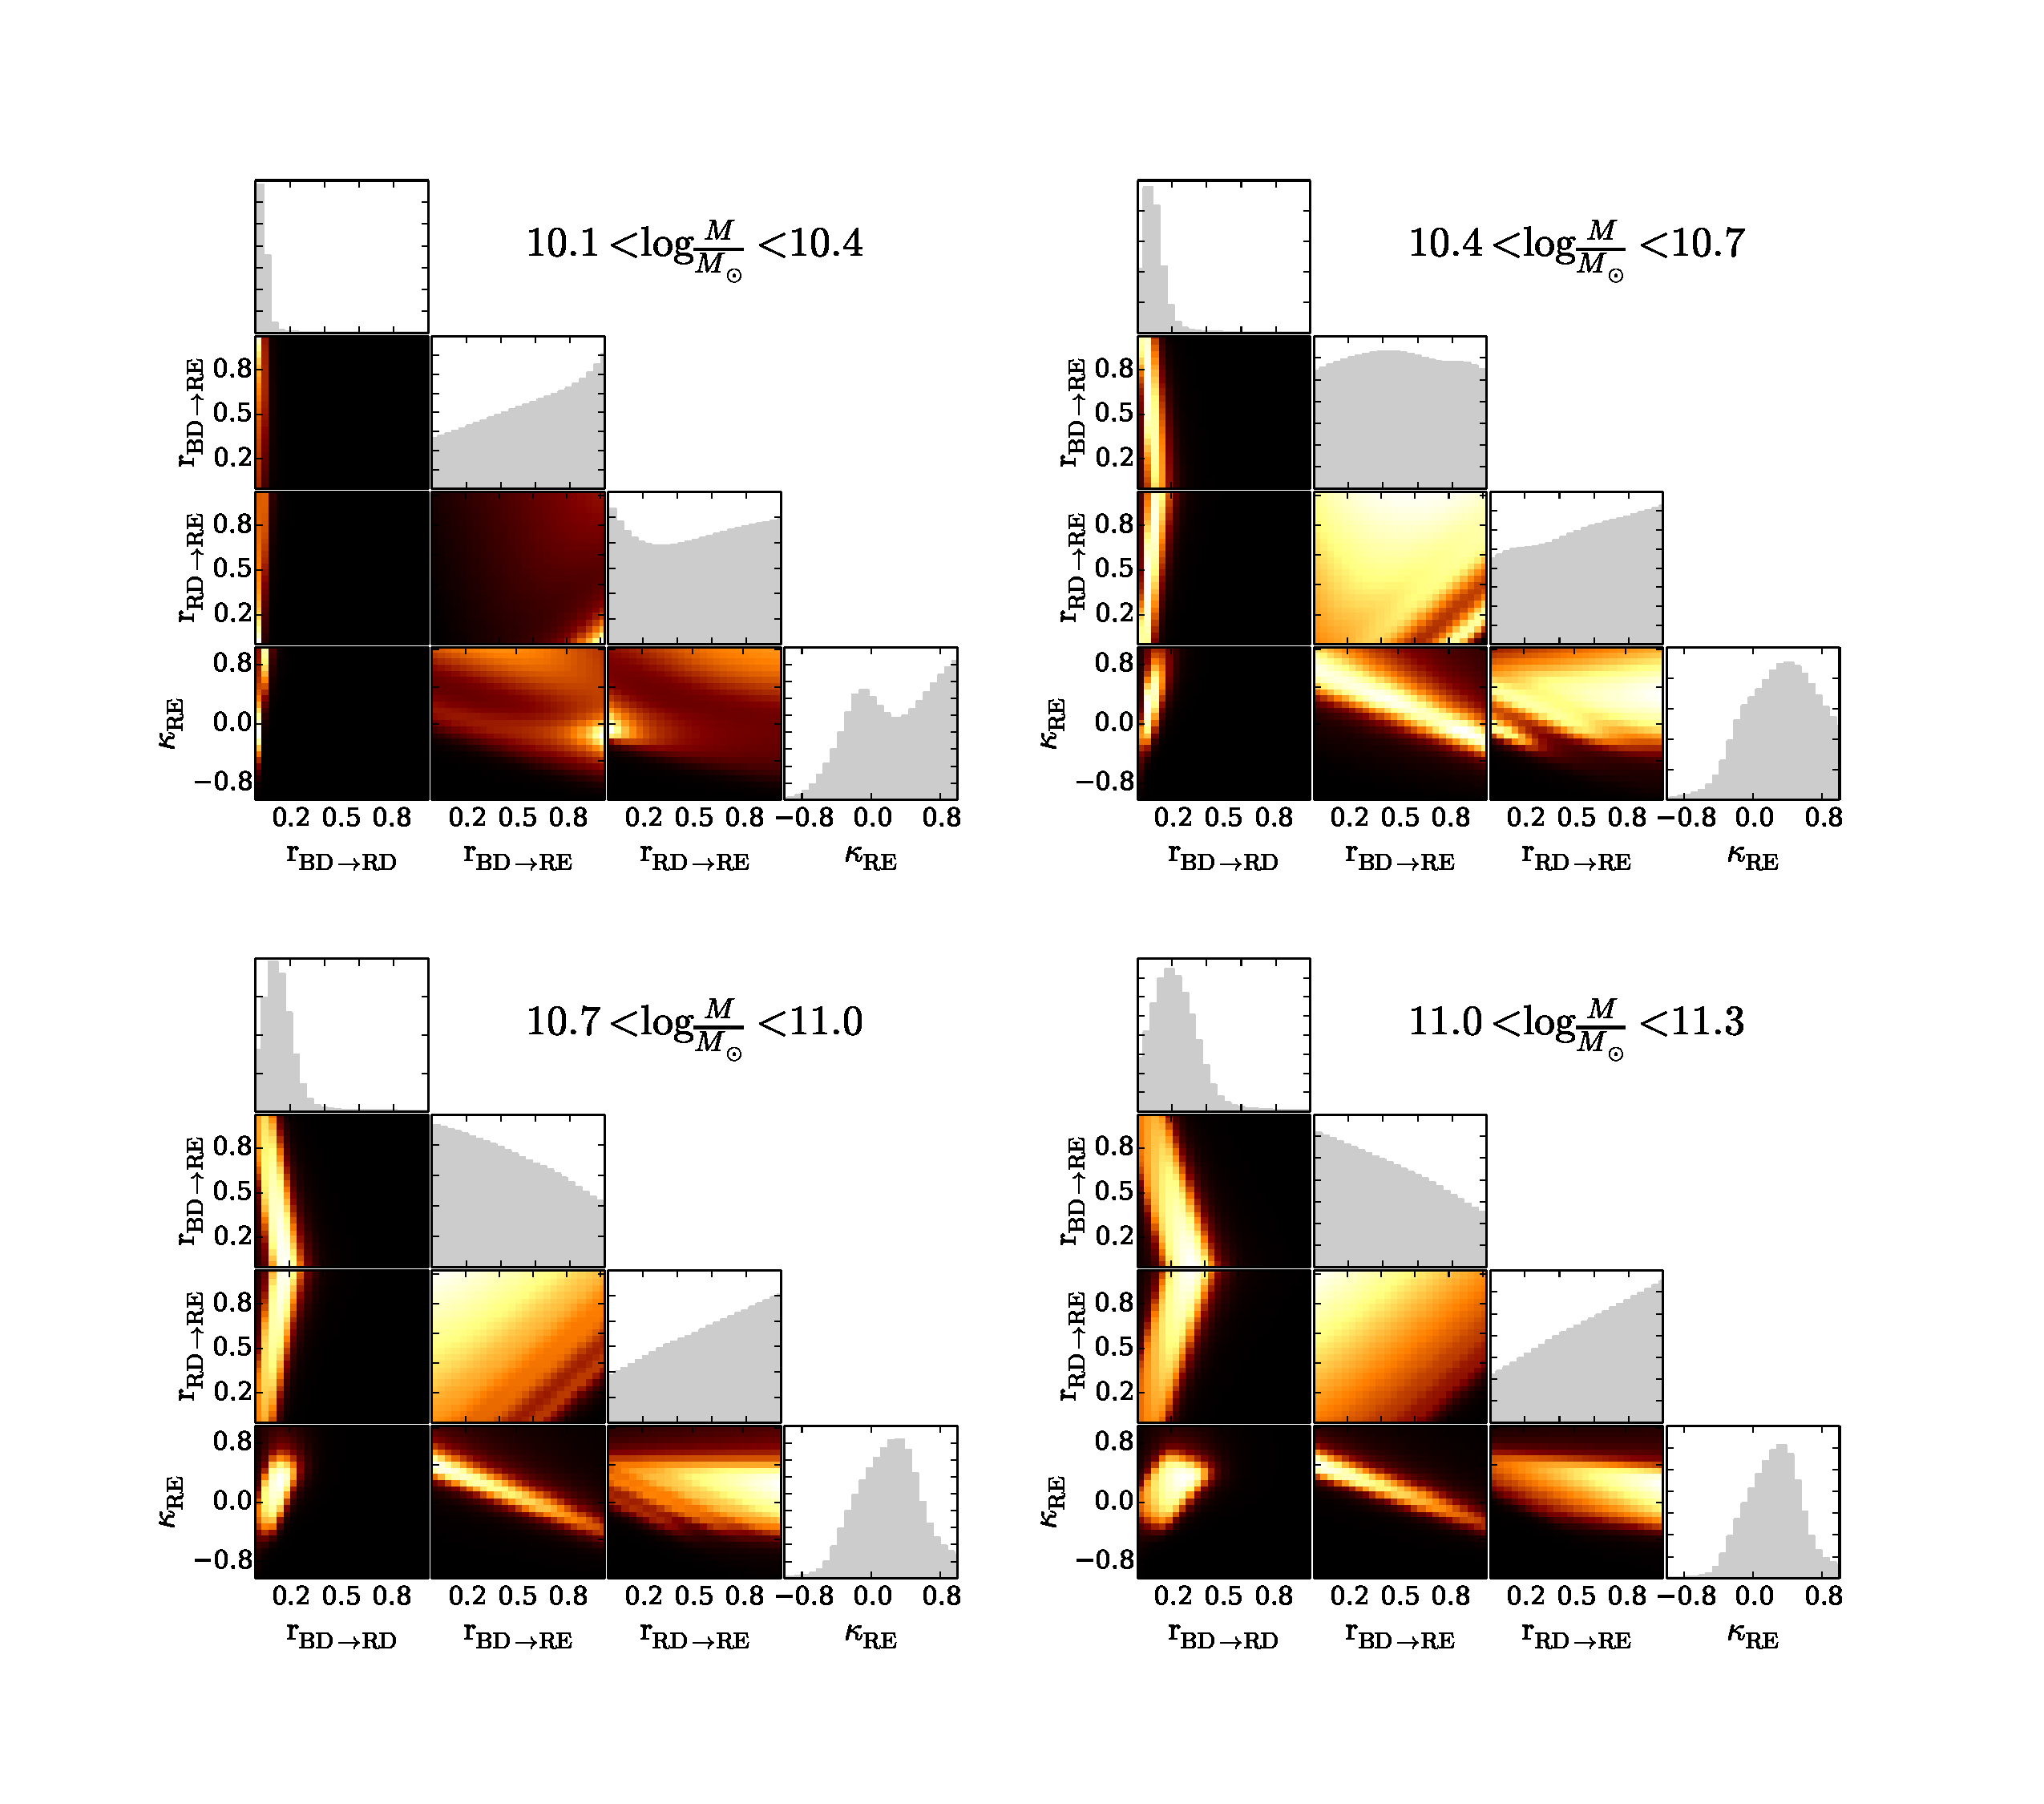
\includegraphics[width=\textwidth,trim={0cm 0cm 2cm 1cm},clip]{figures/corner_plot.pdf}
\caption{Results of the grid-search for the best-fit rate parameters $r_{BD \rightarrow RD}, r_{BD \rightarrow RE}, r_{RD \rightarrow RE}$, and $\kappa_{RE}$ for four mass bins. The units for all rate parameters is $\rm Gyr^{-1}$. 25 equally-spaced values were tested between (0,1) for each parameter, with the exception of $\kappa_{RE}$ which was tested for 25 values between (-1,1); these are represented by the 25 bins on each axis. Each bin is weighted by $1/\chi^2$, such that white regions correspond to parameters which produced the lowest $\chi^2$, and black representing the highest. There is a strong result in the dependence of $r_{BD \rightarrow RD}$ with mass, such that the fraction of blue disks which transition to red disks (ie, quench without disrupting the disk), increases for more massive galaxies. The other parameters are less constrained by this model; therefore a more complex semi-analytic model will be necessary for obtaining the precise values of these rates, and is the subject of future work.}
\label{fig:corner}
\end{figure*} 

We find a strong mass dependence on the fraction of blue galaxies to quench to red disks ($r_{BD \rightarrow RD}$), or Path A in Figure~\ref{fig:cartoon}. Our observations of $f_{R|D}$ and $f_{D|R}$ are most closely reproduced when $r_{BD \rightarrow RD}$ = [0.05, 0.07, 0.1, 0.2] $\rm Gyr^{-1}$ for masses $\rm log(M/M_{\odot})$ = [10.25,10.55,10.85,11.0]. [Note: need to measure peaks explicitely, current values are by-eye. Also calculate 1-sig errors.] These values for $r_{BD \rightarrow RD}$ correspond to the peaks of the 1-D histograms shown in Figure~\ref{fig:corner}. This increase of $r_{BD \rightarrow RD}$ with mass could suggest either: 1) more massive galaxies are more likely to undergo quenching processes which do not destroy their disks, or 2) less massive galaxies simply quench less frequently overall, via any pathway. 


 Analysis of the next parameter in the low mass bin, $r_{BD\rightarrow RE}$, suggests that the former is more likely, given the peak of $r_{BD \rightarrow RE}$ at $>0.9 ~\rm Gyr^{-1}$. The high rate of low-mass blue disks quenching to red ellipticals is evidence that they do not quench any less frequently than high mass galaxies, and the increase of $r_{BD \rightarrow RD}$ with mass is indeed consistent with quenching processes less likely to destroy the disk of massive galaxies. However, this result is not nearly as constrained, given the broad distribution of likelihoods for this parameter. $r_{BD \rightarrow RE}$ is even less constrained for all higher masses. The degeneracies evident in this rate and $r_{RD \rightarrow RE}$ make it clear that our model is not sufficient to constrain the relative fequencies of the processes involved in quenching and morphological transformations; a more sophisticated model with the adjustments we have described thus far would be necessary to paint the full picture. 




\end{document}
